\chapter{Evaluation}\label{eval}%

%\section{Evaluation}

    This chapter delves into the comprehensive evaluation and experimentation phase that forms the cornerstone of this research endeavor. The primary objective is to rigorously assess the proposed software framework's viability, effectiveness, and real-world applicability. A systematic series of experiments and assessments, including three types of evaluations, aims to validate the hypotheses formulated in the earlier stages of this study and provide empirical evidence to support the claims. The chapter unfolds as follows: 
    
    \begin{itemize}
        \item  Section \ref{designTime} outlines the design-time evaluations of the introduced tool, providing an in-depth analysis of the experimental results for various scenarios.
        \item Section \ref{runTime} presents an experimental setup using a real hardware platform and detailing methods and parameters utilized to conduct our evaluations. This section also offers insights into the rationale behind selecting these components and their alignment with real-world scenarios.
        \item  In Section \ref{qualTime}, the focus is shifted towards a qualitative evaluation that offers a nuanced perspective on the introduced tool. Here, the emphasis lies on elucidating how this tool facilitates the design and synthesis of intricate E/E systems. Through this analysis, the tool's potential is uncovered in streamlining the design process and enhancing the synthesis of systems, thus contributing to advancing engineering practices. Moreover, this section undertakes an evaluation of the installation process of the framework, providing a comprehensive assessment of its usability and ease of integration.
    \end{itemize}
    
   
    
    
     %Section III provides an analysis of a qualitative evaluation. This analysis focuses on how the tool can facilitate the design and synthesis of E/E systems. Moreover, the installation process of this framework is assessed.
     
   




    %The ability of the framework to implement a highly model-based TSN configuration isdemonstrated where constraint building, schedule synthesis, and switch configuration arefully automated. We present a proof of concept that highlights how the manual workrequired for TSN configuration is minimized.
    %The developed framework is used to model and configure an experimental setup consisting of prototypical implementation of IEEE 802.1Qbv switches. The latency and jitter of time-triggered streams are measured and analyzed regarding the expectations from IEE 802.1Qbv.

   
    
    \section{Design-time Evaluation}\label{designTime}

    Through diverse case studies, this section assesses the tool's performance, applicability, and scalability in the design phase. The goal is to highlight its strengths, adaptability, and potential areas for improvement, providing empirical insights into its real-world value.

    The proposed framework serves as a valuable asset in streamlining the design process for system architects. However, the practical utility of this framework can be hampered by prolonged computation times involved in both constraint generation and solving processes. To address this challenge, a comprehensive investigation is conducted to discern the impact of various parameters within the presented system model on the time required for efficient constraint set generation and solving~\cite{9565115,askaripoor2023designer}.
    Furthermore, this study includes a meticulous scalability analysis, underscoring the tool's capability to seamlessly accommodate systems of considerable magnitude. This entails an exploration of the novel single-step solving algorithms and formulations, demonstrating their scalability even when dealing with intricately large systems~\cite{askaripoor2023designer}. 
    
    Notably, the \textit{Gurobi 9.5} solver~\cite{gurobi}, as mentioned in Chapter~\ref{method}, is used for effectively solving the system models. It is worth noting that all experiments conducted during the design phase are performed on a laptop equipped with a robust 2.80GHz Core i7 processor and a 16 GB memory capacity. This setup ensures that the experimental conditions align with real-world scenarios while upholding consistent standards throughout the evaluation process.
    
    
    
      %\subsection{Design-time Evaluation of E/E Designer Framework}
    
    %The \textit{E/E Designer} framework facilitates the design process for system architects. Nonetheless, high computation times forgeneration and solving the constraints will have a negative impact on practical usage. Therefore, it is investigated how different parameters of the designed system using the \textit{E/E Designer} affect the time required to generate and solve the constraint set used in the tool. In addition, a scalability analysis is presented and it is shown that the introduced single-step solving algorithms and formulation scale to systems with reasonably large sizes. The \textit{Gurobi 9.5}~\cite{gurobi} is utilized  for solving the system models, as mentioned in Chapter~\ref{method}, and all design-time experiments are executed on a laptop with a 2.80GHz Core i7 processor and 16 GB memory.
    \subsection{Evaluation of Communication Message Routing Generation}
    
    %Our proposed approach facilitates the design process for system architects. Nonetheless, high computation times for generation and solving the constraints will have a negative effect on practical usage. Therefore, this section focuses on measuring the run time of constraint generation and solving for three specific scenarios.
    %In this experiment, only the synthesis time of the constraint set for the communication message routing generation is measured. The synthesis time consists of the time for generating the variables and constraints of the system model and the time for solving the constraint set. This experiment was performed to see how the message routing constraint set itself affects on the synthesis time considering homogeneous redundant paths. Three specific scenarios are considered while all designed topologies/architectures are full-mesh.
    
    This experimental study solely evaluates the synthesis time associated with generating communication message routing constraints concentrating on homogeneous redundant routes. The synthesis time encompasses two fundamental components: the duration required to formulate the system model's variables and constraints and the time to effectively solve the resultant constraint set.
    This investigation is centered around comprehending the direct influence of the message routing constraint set on the synthesis time, particularly in the context of homogeneous redundant paths. The underlying motivation is to dissect how these constraints shape the temporal aspects of the synthesis process. The analysis is performed under four distinctive scenarios, each carefully curated to encapsulate specific conditions and variables~\cite{9565115}.
    It is essential to underline that the chosen experimental scenarios are characterized by deploying fully interconnected topologies or architectures—commonly referred to as full-mesh arrangements as illustrated in Chapter~\ref{method}. This choice allows us to isolate and interrogate the impact of message routing constraints within a controlled environment.
    
    
    
    %In the first scenario, the number of homogeneous redundant (HR) routes is increased while the number of applications and nodes is constant. As the second scenario, the constant number of applications is increased rather than the last scenario and the synthesis time is measured again. In the third scenario, the number of applications increases whereas the number of nodes and HR routes remains constant. In the last scenario, the number of nodes is grown and the number of HR routes and applications remains unchanging. Each measurement consists of two parts: the time for generation of MIP constraints and the time for solving.
    \subsubsection{First Case Study}
    In the first scenario, the count of homogeneous redundant (HR) routes is increased while keeping the number of applications and nodes constant. Moving to the second scenario, the number of applications remains constant but increases compared to the previous scenario, and the synthesis time is subsequently measured. In the third scenario, the number of applications increases while maintaining a constant number of nodes and HR routes. Lastly, the number of nodes is incremented in the fourth scenario, while the count of HR routes and applications remains unchanged. Each measurement comprises two components: the time to generate MIP constraints and the time to solve. It should be added that the cost optimization goal for the communication links was applied during these experiments~\cite{9565115, 9212001}.





    
    %The number of applications  In the second scenario, the number of applications increases whereas the number of nodes and HR routes remains constant. 

    %For the first one,  which include two/forty safety-critical applications as the sender and the receiver  routing one/twenty data ($d\in D_s)$ over the topology where they are mapped on two/forty nodes as the source and the destination respectively. 

    \subsubsection{Second Case Study}
    To assess the impact of increasing the number of HR routes in the synthesis time, refer to Figure~\ref{fig71}~(a); topologies were generated with the same number of nodes and applications, fixed to 100 and 2 respectively, while the number of routes was increased from one to six. As Figure~\ref{fig71}~(a) depicts, the number of HR routes does not significantly influence the constraint generation time in contrast to the solving time, which exhibits a noticeable linear rise. A similar experiment to the last scenario was conducted to observe the effect of the number of applications on HR routes, with the only difference being that the number of applications was altered to 20 instead of 2. As shown in Figure~\ref{fig71}~(b), both the generation and solving times exhibit similar linear trends to the previous scenario; however, the solving process takes considerably longer in this particular experiment~\cite{9565115}.
	
	\begin{figure}[ht]
	\centering
	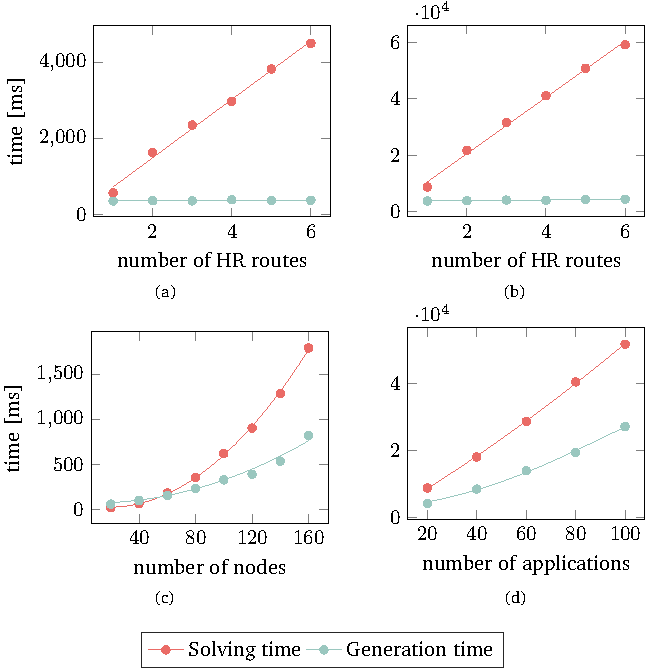
\includegraphics[width=0.8\textwidth]{figures/routing_cropped.pdf}
	\caption{The architectural synthesis times for the defined experimental scenarios involving communication message routing integrated into the E/E Designer tool. The constant variables for each scenario are established as follows: (a) Two applications and one hundred nodes. (b) Twenty applications and one hundred nodes. (c) Six HR paths and two applications. (d) One hundred nodes and six HR paths.}
	\label{fig71}
	\end{figure}
 
          
    %In the third scenario, the number of applications and HR routes are kept constant, 2 and 6 respectively, whereas the number of nodes increases to 160 to observe the node's influence on the synthesis time. As shown in figure~\ref{fig71}~(c), the generation time grows as the number of nodes increases.  Furthermore, it can be seen that the run time shows a non-linear increase. Moreover, figure~\ref{fig71}~(c) exhibits exponential growth in the solving time as the number of nodes increases. As an example, the solving time for 80 nodes is roughly 400 milliseconds while it increases to 1700 milliseconds for 160 nodes~\cite{9565115}. 
    \subsubsection{Third Case Study}
    In the third scenario, the number of applications and HR routes remains constant at 2 and 6, respectively, while the number of nodes increases to 160 in order to observe the influence of nodes on the synthesis time. As depicted in Figure~\ref{fig71}~(c), the generation time expands as the number of nodes increases. Moreover, it is evident that the run-time displays non-linear growth. Furthermore, Figure~\ref{fig71}~(c) illustrates exponential escalation in the solving time as the number of nodes increases. For instance, the solving time for 80 nodes is approximately 400 milliseconds, while it escalates to 1700 milliseconds for 160 nodes~\cite{9565115}.

         
     %For the last scenario, the number of applications is increased from 20 to 100 while the number of nodes and HR routes are fixed at 100 and 6 respectively. The goal is, to investigate the impact of the increase in the number of applications on the constraint generation and solving times. As figure~\ref{fig7}~(d) illustrates, the run time for constraint generation non-linearly rises (approximately from 4500 to 27000 milliseconds) in proportion to the increase in the number of applications, once the number of applications grows from 20 to 100. figure~\ref{fig71}~(d) indicates an increase in the solving time as the number of applications grows and the nodes and number of HR routes remain constant.For example, to solve the constraints of an architecture that consists of 100 nodes and 20 applications supporting six HR routes, the required time is roughly 10 seconds while the architecture comprising 100 applications and the same number of nodes as well as HR routes, requires about 50 seconds~\cite{9565115}. In contrast to figure~\ref{fig71}~(c), the solving time indicates less exponential behavior based on figure~\ref{fig71}~(d).     Note that the number of nodes has less impact on constraint generation and solving times than the number of applications based on figure~\ref{fig71}~(c) and (d).
     
    \subsubsection{Forth Case Study}
     In the final scenario, the number of applications is increased from 20 to 100 while keeping the number of nodes and HR routes fixed at 100 and 6, respectively. The objective is to investigate the impact of the increased number of applications on constraint generation and solving times. As shown in Figure~\ref{fig71}~(d), the run-time for constraint generation non-linearly increases (from approximately 4500 to 27000 milliseconds) in correlation with the growth in the number of applications when transitioning from 20 to 100 applications. Similarly, Figure~\ref{fig71}~(d) illustrates an increase in solving time as the number of applications increases, while the nodes and number of HR routes remain constant.
    For instance, solving the constraints for an architecture with 100 nodes and 20 applications supporting six HR routes takes about 10 seconds. In contrast, the architecture with 100 applications and the same number of nodes and HR routes requires approximately 50 seconds. In contrast to the trend seen in Figure~\ref{fig71}~(c), the solving time displays a less exponential behavior, as depicted in Figure~\ref{fig71}~(d)~\cite{9565115}.
    It is worth noting that, based on Figures~\ref{fig71}~(c) and (d), the number of nodes has a comparatively more minor impact on constraint generation and solving times than the number of applications does.
 
        
        
        
        
     \subsection{Automated Mapping Approach and Application Threads' Scheduling Evaluation}
    
    %In this experiment, the synthesis time for the automated mapping approach integrated into the proposed framework is discovered. This investigation is centered around comprehending the direct influence of the mapping constraint set on the synthesis time. The underlying motivation is to dissect how these constraints shape the temporal aspects of the synthesis process. Note that the analysis is performed under the premise of four distinctive scenarios, each carefully curated to encapsulate specific conditions and variables.It is essential to underline that the chosen experimental scenarios are characterized by the deployment of zonal topologies or architectures. This choice allows to isolate and interrogate the impact of mapping constraints within a controlled environment~\cite{askaripoor2023designer}.

    This experiment explores the synthesis time related to the integrated automated mapping approach and the time-triggered scheduling for mapped application threads within the proposed framework. This investigation focuses on understanding the direct impact imposed by the mapping and scheduling constraint sets on the synthesis time. The primary motive is to dissect how these constraints intricately shape the temporal dimensions of the synthesis process. Notably, this experiment unfolds within the context of four different scenarios. These scenarios were carefully designed to help understand how mapping and scheduling constraints influence the system.
    It is vital to highlight that the selected experimental scenarios involve using zonal topologies or architectures. This specific choice enables isolating and carefully studying the constraints' subtle impacts in a controlled environment~\cite{askaripoor2023designer}.



       \begin{figure}[ht]
    	\centering
    	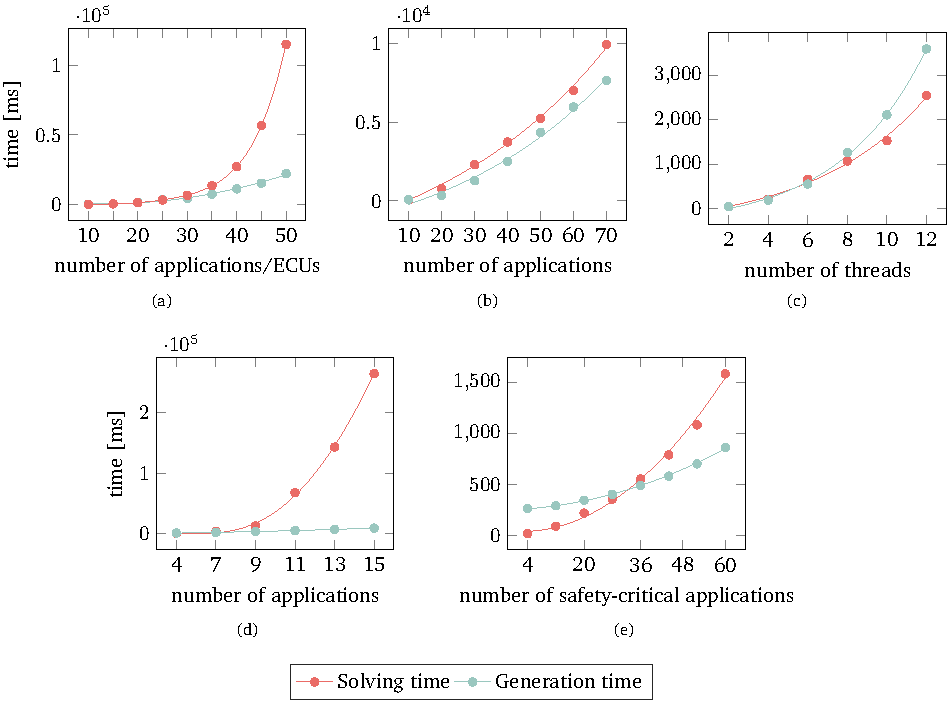
\includegraphics[width=1\textwidth]{figures/results_mapping_scheduling.pdf}
   	\caption{Design-time performance evaluation of the introduced model-based framework. The resource utilization constraint is applied to all use cases. (a) Each application consists of two threads. (b) It is applied on a topology including 8 ECUs, and each application has two threads. (c) The topology consists of 8 applications and 8 ECUs. (d) The topology comprises 8 ECUs, and each application consists of two threads with odd periods.
   	    (e) A zonal architecture including 15 ECUs is applied in this use case, and each safety-critical application has one thread. The boundary goals for resource utilization, maximum memory usage, and safety-critical mapping constraints are applied.}
    	\label{fig72}
        \end{figure} 

    %It is of importance to emphasize that the chosen experimental scenarios are characterized by the deployment of zonal topologies or architectures. This deliberate selection allows to isolate and meticulously examine the nuanced effects of mapping constraints within a tightly controlled environment~\cite{askaripoor2023designer}.


    In the first three case studies, Figures~\ref{fig72}~(a), (b), and (c), the mapping problem is solved by applying the resource utilization (RU) as a hard constraint and the scheduling for threads running on each control node using the E/E Designer framework. Note that in this experiment, the single-step solving algorithms for mapping and scheduling were applied as explained in Chapter~\ref{method}. 
    
    %In the four presented case studies,  the mapping problem is solved by applying the resource utilization (RU) objective as a hard constraint and the scheduling for application threads running on each control node using \textit{E/E Designer}.
    \subsubsection{First Case Study}
    %In the first case study, a distributed E/E system is modeled consisting of 10 applications, each including two threads with random execution times $t_i.e$ and even periods $t_i.p$, and 10 ECUs as control nodes.
    In the initial case study, a distributed E/E system model is constructed comprising ten applications, each encompassing two threads with randomly assigned execution times represented as $t_i.e$, along with even periods denoted as $t_i.p$. Additionally, ten ECUs were employed as control nodes within this setup.
    For the subsequent case study, the system dimensions is extended to encompass fifty applications and ECUs. This expansion allowed to evaluate both the time taken for solving the constraint set and the time needed for generating MIP constraints (as depicted in Figure~\ref{fig72}~(a)). The trend observed in the solving time presents a clear exponential pattern, particularly when the count of applications exceeds thirty~\cite{askaripoor2023designer}.

    %In this case study, the system size is increased from 10 to 50 applications and ECUs to measure solving time of the constraint set and the time for generation of MIP constraints (See figure~\ref{fig72}~(a)). As can be seen, the solving time illustrates an exponential trend, specially when the number of applications are over 30.
    
    \subsubsection{Second Case Study}
    %In the second case study, a distributed system with 8 ECUs and ten applications, each comprising two threads, is designed, and the same constraints and solving options as for the first use case are applied. The number of applications are increased from 10 to 70 while maintaining the number of ECUs constant to observe the timing behavior for the constraint set solving and generation. Based on figure~\ref{fig72}~(b), the solving time rises exponentially as more thread schedules must be calculated for each ECU. For instance, considering 70 applications assigned to 8 ECUs means that each ECU executes at least eight applications or 16 threads (taking RU objective into account), which must have correct schedules.


    In the second case study, the design of a distributed system featuring 8 ECUs and 10 applications, each application comprising two threads, is undertaken. The same constraints and solving options as those used in the first use case are applied. Subsequently, the scope is extended by increasing the number of applications from 10 to 70 while maintaining a consistent number of ECUs. This expansion allows us to keenly perceive the timing behavior during constraint set solving and generation.
    As described in Figure~\ref{fig72}~(b), the solving time reveals exponential growth due to the augmented number of thread schedules that must be computed for each ECU. For instance, when we contemplate allocating 70 applications across the 8 ECUs, it implies that each ECU handles a minimum of eight applications or 16 threads (factoring in the RU objective). Each of these threads necessitates an accurate schedule, thus contributing to the observed trend in the solving time~\cite{askaripoor2023designer}.
    
    \subsubsection{Third Case Study}

     %For the use case shown in figure~\ref{fig72}~(c), the exact measurement with a model including eight applications and 8 ECUs is performed, but in this use case, we only increase the number of threads from 2 to 12 for each application. As figure~\ref{fig12}~(c) shows, exponential growths can be seen for solving and generation times. 
         
    In the context of the use case depicted in Figure~\ref{fig72}~(c), a precise measurement is conducted using a model comprising eight applications and eight ECUs. However, in this specific scenario, the thread count for each application is only increased from 2 to 12. As illustrated in Figure~\ref{fig72}~(c), discernible exponential increments become evident in both solving and generation times~\cite{askaripoor2023designer}.




     
    \subsubsection{Forth Case Study}
    
    %Since finding schedules for several threads with odd periods is more complicated than even periods due to the least common multiplier and the hyperperiod calculations, an use case is defined to observe this statement in action. Therefore, figure~\ref{fig72}~(d) presents the times measured for a system model consisting of 5 ECUs and 4 applications each containing 4 threads. The applications only grow from 4 to 15 while having the same number of threads but with odd periods e.g., 5, 7, 11, and 13. As can be seen, the solving time exponentially rises which proves the complication in schedule computation for the threads whereas the generation time is approximately constant compared to the solving time.
    Since deriving schedules for multiple threads with odd periods is notably more intricate than even periods due to the complexities of least common multiple and hyperperiod calculations, a practical case is formulated to witness this phenomenon firsthand. As a result, Figure~\ref{fig72}~(d) illustrates the observed durations within a system model comprising 5 ECUs and four applications, each housing four threads. The number of applications remains constant, ranging from 4 to 15, with the only variation in the threads' periods, which are odd numbers such as 5, 7, 11, and 13. The graphical representation visually demonstrates the exponential increase in the solving time, substantiating the intricacies involved in computing schedules for threads with odd periods. Conversely, the generation time depicts a relatively consistent trend when juxtaposed with the solving time.
    
    \subsubsection{Fifth Case Study}
    
     %figure~\ref{fig72}~(e) shows measurements for solving a mapping problem and finding correct schedules for application threads. A zonal architecture, similar to figure~\ref{fig5} in Chapter~\ref{evaluation}, was modeled, including 15 ECUs. We increased the number of applications from 4 to 60 while defining all applications, each including one application thread, as safety-critical. During the solving step, ECU usage and maximum memory utilization of each ECU are set as boundary constraints, and further mapping constraints, as explained in the automated mapping conditions such as redundancy for safety-critical applications are involved. Since the safety-critical application must be executed redundantly, in the case of 60 safety-critical applications, 120 applications are running in the topology~\cite{askaripoor2023designer}. 
     
    Figure~\ref{fig72}~(e) illustrates the measurements committed to address a mapping problem and ascertain accurate schedules for application threads. For this purpose, a zonal architecture is employed, similar to the one presented in Figure~\ref{fig5} of Chapter~\ref{frontend}, comprising 15 ECUs. The range of applications is expanded from 4 to 60, each flagged as safety-critical, encompassing a single application thread.
    During the solving phase, boundary constraints were established for ECU utilization and maximum memory usage on each ECU. Furthermore, supplementary mapping constraints were incorporated, as delineated within the automated mapping conditions, including redundancy provisions in safety-critical applications. It is crucial to emphasize that owing to the requisite redundancy when dealing with 60 safety-critical applications, a total of 120 applications are concurrently executed within the topology~\cite{askaripoor2023designer}.
     
           \begin{figure}[ht]
    	\centering
    	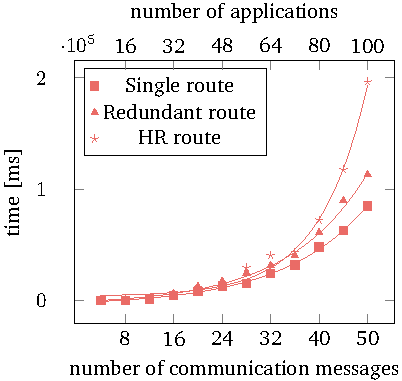
\includegraphics[width=0.5\columnwidth]{figures/full-framework.pdf}
   	\caption{The measurement of solving time in a case study includes the full capabilities of the proposed tool while considering different types of paths for transferring communication messages. The same architecture as in Figure~\ref{fig72}~(e) is used in this experiment. This study incorporates the multi-objective optimization, which encompasses end-to-end latency, response time, and LOR, as well as the goals for resource utilization and maximum memory usage~\cite{askaripoor2023designer}.}       
   	
   	%In this use case, the vehicle topology has 8 ECUs and each application has two threads with odd periods. A centralized architecture that includes links and 17 ECUs, and each application includes two threads. The multi-objective optimization, including end-to-end latency and response time, is applied to this use case.}
    	\label{fig73}
        \end{figure} 
    
    \subsection{Evaluation of Full Capabilities of the E/E Designer Framework in a Single-Step Solving}
         
    %In this experiment, the full capabilities of the tool are assessed while taking single step solving algorithms such as CMR, CSCT, and PD, as illustrated in Chapter~\ref{method}, into account. In the this use case, the automatic message routing and mapping, the threads and communication tasks schedulings, and path and message dependencies are solved in a single-step while applying various optimization objectives and boundary constraints. Besides, the influence of the creation of various types of paths on the solving time while applying the other aforementioned features is investigated.
    
    In this experiment, the complete capabilities of the tool are assessed, incorporating single-step solving algorithms like CMR, CSCT, and PD, as detailed in Chapter~\ref{method}. In this particular use case, the experiment encompasses automatic message routing and mapping, time-triggered scheduling of threads and communication tasks, and resolving path and message dependencies, all within a single step. Various optimization objectives and boundary constraints are applied during this process. In addition, the impact of creating different types of paths on solving time while employing the features mentioned above is investigated. This investigation aims to comprehensively understand how the interplay between route types, communication volume, and application count manifests in the solving time dynamics. This analysis serves as a crucial step in assessing the efficiency and scalability of the introduced approach within a representative zonal E/E architecture~\cite{askaripoor2023designer}.



     %In figure~\ref{fig73}, we investigate the influence of the creation of various types of routes on the solving time while applying automatic mapping and the application threads and communication tasks schedulings in a single-step for the same zonal E/E architecture modeled in figure~\ref{fig72}~(e). We measure the solving time for creating three types of routes: single, redundant, and HR paths (generating three disjoint routes) from senders to receivers (chosen automatically based on mapping constraints) while increasing the number of communication messages from 4 to 50 and applications from 8 to 100 (each including one thread). 
    
    
     Figure~\ref{fig73} explores the impact of generating various route types on the solving time. This study involves the application of automatic mapping, alongside scheduling application threads and communication tasks within a single step, all within the context of the same zonal E/E architecture depicted in Figure~\ref{fig72}~(e). The focal point of our investigation is to gauge how the creation of distinct routes influences the time required for solving.
     The solving time is quantified across three distinct route types, including single, redundant, and HR paths, each responsible for generating three independent routes. These routes are automatically determined based on mapping constraints. Concurrently, the number of communication messages is systematically varied from 4 to 50, and the count of applications is increased from 8 to 100. Each of these applications encompasses a single thread~\cite{askaripoor2023designer}.
     
     
     
     
     
     Moreover, the multi-objective optimization is applied, as illustrated in Chapter~\ref{method}, including end-to-end latency, response time, and LOR. This optimization uses a hierarchical methodology, with RU and maximum memory usage acting as single boundary objectives.
     To illustrate, consider Figure~\ref{fig73} as an example. In scenarios involving 50 communication messages and 100 applications, the solution consists of a variety of 50 paths. These paths include single, redundant, and HR routes, all carefully constructed from senders to receivers. These solutions also comprise task schedules over links solely for activated routes and application-to-ECU mappings and thread schedules on each individual ECU~\cite{askaripoor2023designer}.
     
    %As expected, the number of generated routes can affect the solving time. Consequently, based on figure~\ref{fig73}, the HR path requires more time as it needs to find three disjoint routes in each scenario. Similarly, a redundant route has higher solving time than a single route (See figure~\ref{fig73}).
    
    As anticipated, the number of generated routes can impact the solution time. Therefore, referring to Figure~\ref{fig73}, the HR path necessitates more time due to the requirement of identifying three distinct routes in each scenario. Similarly, a redundant route exhibits a longer solving time than a single route (see Figure~\ref{fig73}).





    %for a zonal E/E architecture model including 17 ECUs, 12 communication messages, and 12 applications each comprising two threads while applying multi-objective optimization (including end-to-end latency and response time) using hierarchical approach and RU objective. All threads have random execution times and even periods. Similarly, the frame lengths of tasks are chosen randomly and their periods are random even values. We increase the number of messages and applications from 12 to 30 while the threads and ECUs remain the same to measure the solving and generation times. As figure~\ref{fig12}.(e) depicts, the solving time remains linear by having 30 messages and 30 applications which is extremely reasonable for such problems as scheduling and routing are NP-hard problems~\cite{atallah2019routing} by using our single-step solving approach. In other words, the solution consists of 30 paths created from senders to receivers, the schedules of tasks over links only for activated routes, the mapping of applications to ECUs, and the thread schedules on each ECU.
    
    
    %In the last use case, the automatic message routing and mapping, and the threads and communication tasks schedulings are solved in a single-step for a zonal E/E architecture model including 17 ECUs, 12 communication messages, and 12 applications each comprising two threads while applying multi-objective optimization (including end-to-end latency and response time) using hierarchical approach and RU objective. All threads have random execution times and even periods. Similarly, the frame lengths of tasks are chosen randomly and their periods are random even values. We increase the number of messages and applications from 12 to 30 while the threads and ECUs remain the same to measure the solving and generation times. As figure~\ref{fig12}.(e) depicts, the solving time remains linear by having 30 messages and 30 applications which is extremely reasonable for such problems as scheduling and routing are NP-hard problems~\cite{atallah2019routing} by using our single-step solving approach. In other words, the solution consists of 30 paths created from senders to receivers, the schedules of tasks over links only for activated routes, the mapping of applications to ECUs, and the thread schedules on each ECU.
    
     \begin{figure}[ht]
    	\centering
    	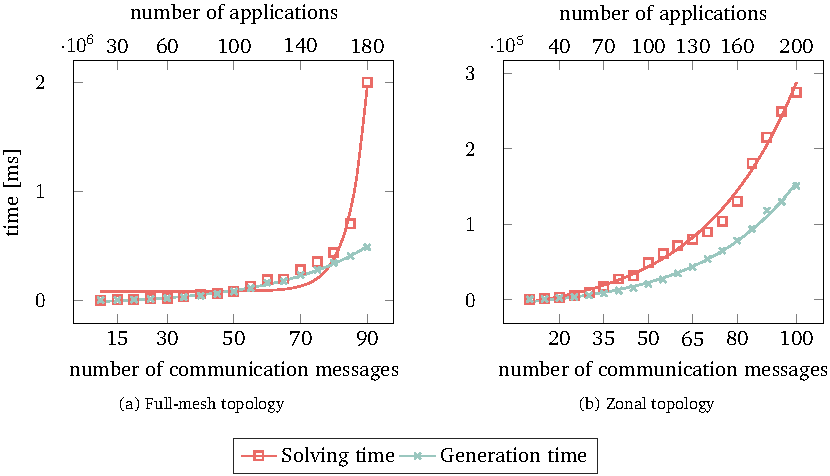
\includegraphics[width=1\columnwidth]{figures/Scalability_analysis.pdf}
   	\caption{Scalability analysis of the presented computer-aided tool. Generation and solving times for (a) a full-mesh architecture and (b) a zonal topology, each including 15 ECUs~\cite{askaripoor2023designer}.} 
   		\label{fig74}
        \end{figure}
        
    \subsection{Scalability Analysis}

      %To evaluate the scalability of the \textit{E/E Designer}, we measure the time required to generate the system model variables and solve the constraint set for two different architectures, such as a full-mesh topology and a zonal topology, each including 15 ECUs. The automatic message routing (for generating single paths) and mapping, as well as the application threads and communication tasks schedulings, are solved in a single step for these two architectures. In addition, we apply the multi-objective optimization, including end-to-end latency, response time, and LOR, and the RU and maximum memory utilization as boundary single objectives. All threads have identical execution times and periods. Similarly, the frame lengths of communication tasks are the same, and their periods are as same as the values of their senders' and receivers' periods. 

      In order to assess the scalability of the proposed framework, an evaluation comprising diverse aspects is conducted. The main objective is to evaluate the time required to generate system model variables and the subsequent resolution of the associated constraint set. This evaluation is performed on two distinct architectural paradigms: a comprehensive full-mesh topology and a more streamlined zonal topology. Each of these architectures comprises 15 ECUs. 
      The introduced tool showcases its prowess within this evaluation by seamlessly handling various intricate tasks. The automatic routing of messages, leading to the generation of single paths, mapping, and scheduling application threads and communication tasks, are all adeptly solved in a single step for both the full-mesh and zonal architectures.
      
      To further enrich the analysis, a multi-objective optimization approach comes into play. This approach considers goals, including the end-to-end latency, the response time, and the LOR. Moreover, the RU and the maximal memory usage serve as boundary objectives, effectively guiding the optimization process. Every application thread shares the exact execution times and periods. Likewise, the frame lengths of communication tasks are equal, with their periods aligned to match the time values of their corresponding senders' and receivers' periods.


      %Our focus lies on gauging the time needed for both generating system model variables and solving the associated constraint set. 






      
      
        
        

      
      %Based on figure~\ref{fig74}~(a), for the full-mesh topology, we increase the number of messages from 10 to 90 and applications from 20 to 180, each comprising an application thread. While, for a zonal topology in figure~\ref{fig74}~(b), the messages rise to 100 and applications to 200. 
       %This means that the \textit{E/E Designer} creates 100 routes from senders to receivers, including their schedules. As figure~\ref{fig74} depicts, the solving time for both use cases grows exponentially.
       %Moreover, as expected, the solving time for the full-mesh topology is significantly higher than that of the zonal one due to the larger exploration space.
        Referring to Figure~\ref{fig74}~(a), in the case of the full-mesh topology, the message count is expanded from 10 to 90, along with the number of applications growing from 20 to 180, each equipped with its dedicated application thread. Meanwhile, as depicted in Figure~\ref{fig74}~(b) for the zonal topology, the number of messages escalates to 100 while the applications increase to 200.
        This implies that the illustrated framework generates 100 routes along with their schedules, spanning from senders to receivers. As illustrated in Figure~\ref{fig74}, the solving time for both scenarios experiences exponential growth.
        Furthermore, as expected, the full-mesh topology's solving time is notably longer than the zonal topology's. This is attributed to the larger space of exploration involved.
      %Considering the zonal topology in figure~\ref{fig74}~(b) and its scale up to 100 communication messages and 200 applications, the solving time is reasonable for problems such as mapping, scheduling, and routing, which are known to be NP-hard problems~\cite{atallah2019routing}, using our single-step solving approach. In practice, the illustrated values are appropriate for an automotive application domain~\cite{askaripoor2023designer}.
        Looking at the zonal topology shown in Figure~\ref{fig74}~(b) and its expansion to accommodate 100 communication messages and 200 applications, the time taken for solving problems like mapping, scheduling, and routing is reasonable. These tasks are recognized as NP-hard problems~\cite{atallah2019routing}, but the introduced single-step solving approach handles them effectively. Notably, the values showcased here are well-suited for real-world applications in the automotive domain~\cite{askaripoor2023designer}.





    
    
    \subsection{Discussion}
        
    %The experimental results during the design phase demonstrate that our formulation and approach enable users to synthesize their desired system model that supports mapping, routing, and scheduling within a reasonable time frame while meeting predefined requirements. Furthermore, applying single and multi-objective optimizations can solve more complex problems and conditions. 
    The outcomes of the experiments in the design stage vividly illustrate the efficacy of the aforementioned formulation and approach. It allows users to efficiently create their intended system models, including mapping, routing, and scheduling, all within a commendable time frame and following predetermined criteria. Moreover, the integration of single and multi-objective optimizations empowers the resolution of intricate challenges and diverse scenarios.
    It is significant to emphasize that the model-based tool, the E/E Designer, is suitable for synthesizing any type of vehicle E/E architecture and network topology, including various configurations of applications, threads, and communication tasks.
    
    
    
    %To evaluate the scalability of \textit{E/E Designer}, we model a centralized architecture comprising 40 ECUs, 50 applications (each having two threads and in total 100 threads), and 40 communication messages. All the periods, execution times, and frame lengths are randomly chosen, and the multi-objective optimization and the RU goals are applied. To solve this system model, \textit{E/E Designer} requires 59 seconds which is a reasonable amount of time, and in practice, the illustrated values are appropriate for many application domains such as automotive.
    
    %The design-time experimental results show that our formulation and approaches allow the user to synthesize its desired system model supporting mapping, routing, and scheduling in a considerable amount of time while fulfilling predefined requirements. In addition, applying single and multi-objective optimizations can figure out more complex problems and requirements. It should be added that \textit{E/E Designer} is applicable to synthesize any type of vehicle E/E architecture, and network topology, including various configurations of applications, threads, and communication tasks.  
 

    \section{Run-time Evaluation}\label{runTime}
    
    As mentioned in the previous section, the framework's performance and applicability are evaluated. In this section, the solutions computed by the tool are deployed on a real hardware platform to observe the applicability of the design-time solutions in a real-world implementation.
    Within the scope of this section, the solutions meticulously calculated by the tool find tangible expression through deployment on an actual hardware platform. This strategic deployment serves as a bridge, connecting the realm of design-time decisions with the dynamic environment of run-time execution. By doing so, it aims to explore how the design-time solutions seamlessly integrate with and translate into practical outcomes during active operational scenarios.
    %As highlighted in the preceding section, a comprehensive evaluation is undertaken to assess both the performance and practical applicability of the framework. Building upon this evaluative foundation, we now transition to a pivotal phase where theoretical propositions are put to the test within the realm of real-world implementation.
    %Within the scope of this section, the solutions meticulously calculated by the tool find tangible expression through deployment on an actual hardware platform. This strategic deployment serves as a bridge, connecting the realm of design-time decisions with the dynamic environment of run-time execution. By doing so, we aim to explore the extent to which the design-time solutions seamlessly integrate with and translate into practical outcomes during active operational scenarios.
    %The deployment onto real hardware platform not only serves as a validation process but also adds a layer of dynamism to our understanding. It unveils how the theoretical constructs, meticulously crafted during design, interact with the actual hardware components and operational conditions. This interplay between theory and practice offers valuable insights into the real-world feasibility and robustness of the solutions.
    In essence, this hands-on deployment provides an opportunity to assess the framework's efficacy in real-world contexts. As it is witnessed the design-time solutions unfolding in real-time scenarios, it gains a more comprehensive understanding of their adaptability, performance, and practical utility. This experiential approach contributes to the holistic assessment of the framework, bridging the gap between concept and implementation~\cite{askaripoor2023designer, 9613692}. 
    
    

    %This section describes how the design-time solutions calculated by the \textit{E/E Designer} were evaluated experimentally on real hardware. For the experiments, three different hardware platforms commonly found in automotive systems were used.
    
    \subsection{Hardware Platform Analysis}
    
    As explained previously, the automotive E/E architecture is shifting towards a centralized architecture, necessitating high-performance computing units capable of processing vast amounts of data. In order to make an informed choice for selecting a vehicle centralized computer or a HPCU, a hardware analysis is conducted~\cite{9613692, askaripoor2022architecture}.




    
    
    
    %Our proposed platform consists of an \emph{AHPCC} having two sub-modules such as software (SW) and hardware (HW). The SW comprises applications, real-time operating systems (RTOS), and middleware whereas the HW comprises a multi-core processor, Graphics Processing Unit (GPU), actuators, and sensors. The \textit{AHPCC} module acts as the center of our proposed platform sending its system properties and requirements to the \textit{E/E Designer}. Accordingly, SW/HW mapping, calculated by the \textit{E/E Designer}, is deployed on the \textit{AHPCC} (See Figure. \ref{fig1}). Finally, the \textit{AHPCC} sends values of the mapping-related parameters to the \textit{Monitoring System} after SW/HW mapping deployment as demonstrated in Figure. \ref{fig1}. There are several AHPCCs, which have been developed by different companies, that we introduce the most relevant products to our work in the following.

    Figures~\ref{fig75}~(1) and~(2) showcase the Drive AGX Xavier and Pegasus Developer Kits, respectively. These kits are designed to provide a comprehensive suite of standard software, hardware, and sample applications tailored to develop self-driving vehicles. Notably, they support diverse input/output (I/O) interfaces, including cameras, LiDAR, radar, and vehicle I/O.
    Both of these kits are equipped with two Xavier SoCs, each capable of accommodating six distinct processor types. These encompass a CPU boasting eight cores, a GPU, a deep learning accelerator (DLA), a programmable vision accelerator (PVA), an image signal processor (ISP), and a stereo/optical flow accelerator.
     The Pegasus Developer Kit shown in Figure~\ref{fig75}~(2) leverages the computational power of additional Turing GPUs, enabling it to achieve an elevated tera operations per second (TOPS) rate \cite{NVIDIA,9613692}.
    %The software stack of the DRIVE AGX Xavier includes sample applications, a software development kit (SDK), an embedded real-time operating system (RTOS), and a hypervisor. Nvidia provides a preconfigured firmware package but restricts information about the platform development kit (PDK) to industrial partners. Nvidia's proprietary hypervisor is therefore not suitable for use in academia.
   The DRIVE AGX Xavier software stack comprises sample applications, a software development kit (SDK), an embedded RTOS, and a hypervisor. Although Nvidia offers a preconfigured firmware package, it limits industrial partners' access to platform development kit (PDK) details. As a result, Nvidia's proprietary hypervisor is not applicable for academic use.





    
    
    %Figure. \ref{fig75}~(1) and \ref{fig75}~(b) demonstrated\textit{DRIVE AGX Xavier} and \textit{Pegasus Developer Kits}, respectively. It is claimed to provide standard software, hardware, and sample applications for the development of self-driving vehicles. They support various input (I)/output (O) interfaces, such as camera, lidar, Radar, and vehicle IO. Both kits have two Xavier systems-on-a-chip (SoCs) that can cover six various types of processors, such a CPU (including 8 cores), GPU, Deep Learning Accelerator (DLA), Programmable Vision Accelerator (PVA), Image Signal Processor (ISP), and stereo/optical flow accelerator. Besides, Pegasus (figure~\ref{fig75}~(b)) employed the power of other Turing GPUs to achieve a higher tera operations per second (TOPS) rate \cite{NVIDIA}.


    %\textit{MPPA-DEV4} development platform, indicated in Figure. \ref{fig2}. (c), can be considered as another vehicle central computer. It prepares a ready-to-use environment to evaluate, develop, and optimize applications in automotive, data-centric, robotics, and communication domains \cite{KALRAY}. Figure. \ref{fig2}. (d) described \textit{R-Car H3} and \textit{M3 Starter Kits} for supporting automotive software development. Also, the process of establishing open-source automotive Linux environments was facilitated by these products \cite{RENESAS}.
    
    The MPPA-DEV4 development platform, as depicted in Figure~\ref{fig75}~(3), serves as another central computer within the vehicle. This platform provides a readily available environment for evaluating, developing, and optimizing applications across domains such as automotive, data-centric, robotics, and communication \cite{KALRAY}. Similarly, Figure~\ref{fig75}~(4) introduces the R-Car H3 and M3 Starter Kits, designed to bolster automotive software development. These products have played a pivotal role in facilitating the establishment of open-source automotive Linux environments \cite{RENESAS,9613692}.
    AVA3501 is a computing platform designed for autonomous vehicles, featuring components like the Intel Xenon 9th Gen CPU and RTX8000 GPU (refer to Figure~\ref{fig75}~(5)) \cite{AVA}. The last associated HPCU, named Nuvo7208VTC, is equipped with an 8-core processor (see Figure~\ref{fig75}~(6)) \cite{Nuvo}.
    
    \begin{figure}[ht]
    \centering
    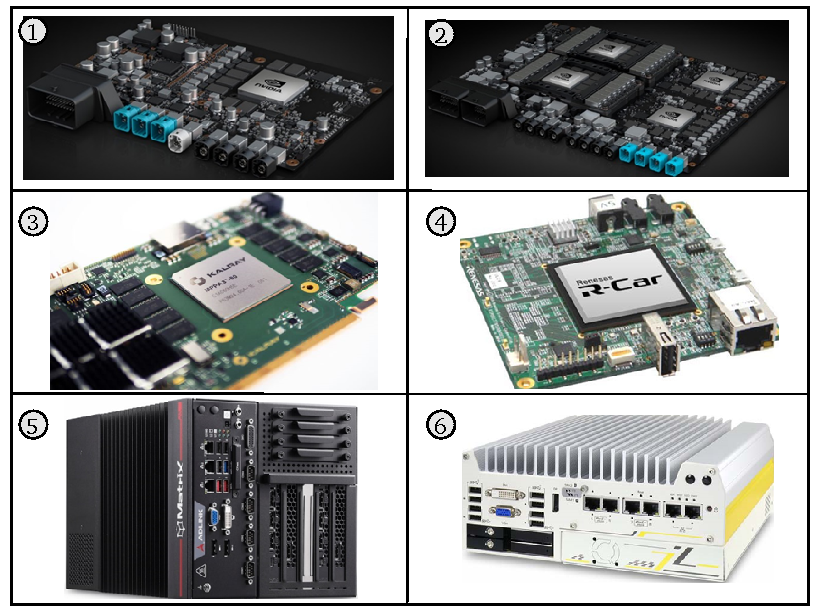
\includegraphics[width=1\columnwidth]{figures/HW_analysis.pdf}
    \caption{The six relevant development kits serve as an HPCU including (1) Nvidia Drive AGX Xavier, (2) Nvidia Pegasus, (3) MPPA-DEV4 development platform, (4) R-Car H3 and M3 Starter Kits, (5) AVA 3501, (6) Nuvo 7208VTC.}
    \label{fig75}
    \end{figure}
    
    Drawing upon the analysis provided above,
    several critical factors informed the decision-making process. These factors encompass computational power, the number of cores, the spectrum of automotive applications, the diversity of interfaces, the quality of customer support, and the comprehensiveness of documentation. Within these considerations, Nvidia AGX Drive emerged as the chosen HPCU for the envisaged hardware platform, primed for in-depth run-time evaluation.
    The capabilities offered by Nvidia AGX Drive align seamlessly with the demanding requirements of the introduced evaluation. Its computational may, augmented by a robust core count, promises a solid foundation for the real-time processing of intricate automotive tasks. The array of interfaces it offers caters to the multifaceted connectivity needs of modern automotive systems.
    Furthermore, the availability of substantial customer support and well-documented resources adds a layer of reliability and ease to the operational endeavors. With Nvidia AGX Drive at the helm, the proposed hardware platform appeared poised for an insightful run-time assessment~\cite{9613692,askaripoor2023designer}.

    %Considering the analysis provided above, which takes into account factors such as computational power, the number of cores, the range of automotive applications and interfaces, customer support, and documentation, Nvidia AGX Drive was determined to be the suitable choice for the High-Performance Computing Unit (HPCU) within the proposed hardware platform employed for run-time evaluation.

    Nonetheless, it is important to note that due to technical considerations linked to Nvidia, as elaborated upon in the subsequent subsections, an alternative development kit was also subjected to testing and subsequent comparison with the Nvidia solution.

    
    
     %Taking above-explained analysis into consideration, based on the computational power, core's number, variety of automotive applications and interfaces, customer support, and documentation, Nvidia AGX Drive was chosen as the HPCU in the proposed hardware platform used for run-time evaluation.
     %However, due to technical reasons related to the Nvidia, which will be explained in the following subsections, other development kit is also tested and compared to the Nvidia.
    \subsection{Experimental Setup}
    
    %This subsection describes how the design-time solutions calculated by the \textit{E/E Designer} tool were evaluated experimentally on real hardware platform. For the experiments, three different hardware platforms commonly found in automotive systems were used. As the main hardware platform or HPCU, the Nvidia Drive AGX Xavier Developer kit was used as it is a popular choice for an HPCU in autonomous driving. The development kit is built around two Xavier SoCs that comprise an 8-core ARM CPU, RAM, and hardware accelerators for deep-learning inference as illustrated in the previous subsection. It runs a modified version of Ubuntu 18.04 with the Preempt-RT-patch as OS. Secondly, experiments were conducted on an Intel i210-based evaluation board to simulate a communication network gateway~\cite{Intel}. Thirdly, a Discovery kit with an STM32L476VG microcontroller was utilized as an example of an energy-efficient ECU~\cite{STM}.
    
    
    This subsection outlines the experimental evaluation of the design-time solutions computed by the proposed tool as they were deployed on real hardware platforms. The experiments encompassed utilizing three distinct hardware platforms commonly featured in automotive systems.
    
    \begin{figure}[t]
    \centering
    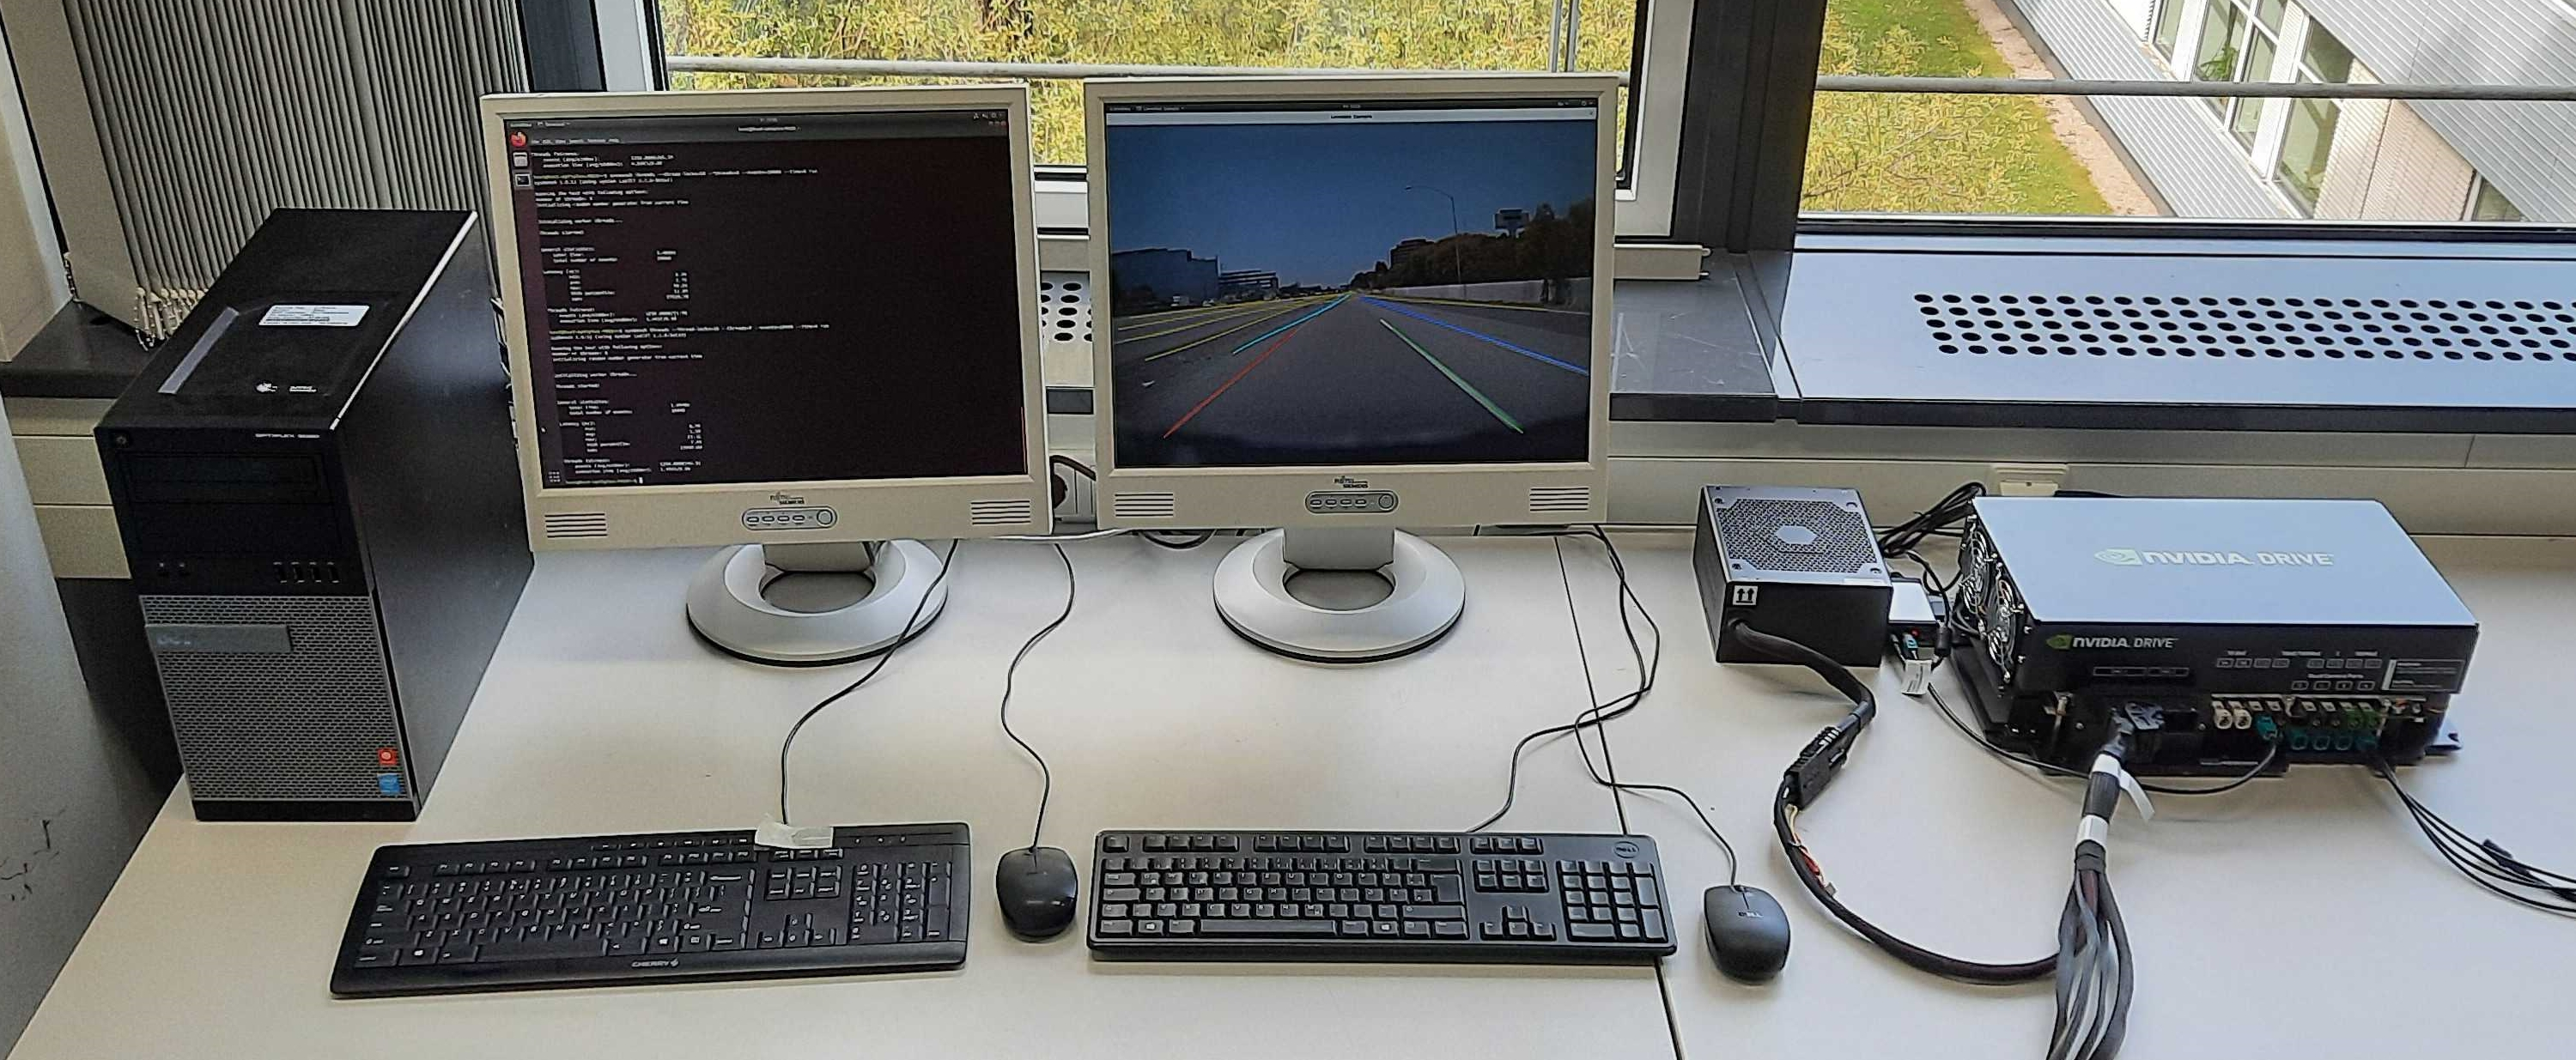
\includegraphics[width=1\columnwidth]{Experimental_setup_2.jpg}
    \caption{The mapping experimental setup using the Nvidia Drive AGX. On the left is the host computer, and on the right is the Nvidia Drive AGX Xavier with the power adapter. Both are connected to a monitor and other peripherals.}
    \label{fig76}
    \end{figure}

    The primary hardware platform chosen for these experiments was the Nvidia Drive AGX Xavier Developer kit, which stands as a prominent selection for HPCUs in autonomous driving (see Figure~\ref{fig76}). This kit revolves around two Xavier SoCs, each encompassing an 8-core ARM CPU, RAM, and hardware accelerators tailored for deep-learning inference, as illustrated in the previous subsection. This platform orchestrates a modified version of Ubuntu 18.04 integrated with the Preempt-RT-patch as its operating system.
    In addition to the Nvidia platform, a series of experiments were conducted on an evaluation board grounded on the Intel i210, effectively simulating the functionality of a communication network gateway~\cite{Intel}. Lastly, a Discovery kit featuring an STM32L476VG microcontroller was harnessed to exemplify an energy-efficient ECU~\cite{STM}.
    This triad of hardware platforms collectively forms the foundation for empirically assessing the framework's design-time solutions~\cite{askaripoor2023designer}.
    
    %The amalgamation of these diverse hardware platforms within our experimental framework bestows a holistic view into the performance and feasibility of the design-time solutions calculated by the \textit{E/E Designer} tool in real-world hardware contexts.
    
    
    
    
    
    
    
    %This subsection outlines the experimental evaluation of design-time solutions computed using the \textit{E/E Designer} tool on tangible hardware platforms. The experimentation involved the utilization of three distinct hardware platforms, commonly encountered within automotive systems.As the primary hardware platform, the Nvidia Drive AGX Xavier Developer kit was selected. Renowned for its significance in the realm of autonomous driving, this platform features the Nvidia Drive AGX Xavier system-on-chip (SoC). Boasting an 8-core ARM CPU, RAM, and dedicated hardware accelerators for deep-learning inference, this platform stands as a prevalent choice for High-Performance Computing Units (HPCUs) within the autonomous driving landscape. The development kit operates on a tailored iteration of Ubuntu 18.04, supplemented with the Preempt-RT patch for enhanced real-time capabilities.Complementing this, experiments were executed on an Intel i210-based evaluation board, chosen for its aptitude in emulating communication network gateways. Additionally, a Discovery kit equipped with an STM32L476VG microcontroller was employed to exemplify an energy-efficient Electronic Control Unit (ECU)~\cite{STM}. This triad of hardware platforms collectively forms the foundation for the empirical assessment of the \textit{E/E Designer}'s design-time solutions.
    
    
    
    
    
    %This section describes how the design-time solutions calculated by the \textit{E/E Designer} were evaluated experimentally on real hardware. For the experiments, three different hardware platforms commonly found in automotive systems were used. First, an Nvidia Drive AGX Xavier Developer kit was chosen because it is a popular choice for an HPCU in autonomous driving. The development kit is built around two Xavier SoCs, each comprising an 8-core ARM CPU, RAM, and hardware accelerators for deep-learning inference. It runs a modified version of Ubuntu 18.04 with the Preempt-RT-patch as the operating system.Secondly, experiments were conducted on an Intel i210-based evaluation board to simulate a communication network gateway~\cite{Intel}.Thirdly, a Discovery kit with an STM32L476VG microcontroller was utilized as an example of an energy-efficient ECU~\cite{STM}.
    
    \paragraph{Reference computer:}
    As a reference based on Figure~\ref{fig76}, a standard computer with an Intel Core i7-4770 @ 3.90 GHz processor with eight cores, 16384 MB of DDR3 memory, a 500 GB disk, and an NVIDIA GeForce GTX 645 graphics card with 1024 MB was used. In addition, all performance tests ran on the Nvidia Drive natively to determine the actual overhead produced by the hypervisor configurations.
    
    
    %First, an Nvidia Drive AGX Xavier Developer kit was chosen because it is a popular choice for an HPCU in autonomous driving. The development kit is built around two Xavier SoCs, each comprising an 8-core ARM CPU, RAM, and hardware accelerators for deep-learning inference. It runs a modified version of Ubuntu 18.04 with the Preempt-RT-patch as the operating system.Secondly, experiments were conducted on an Intel i210-based evaluation board to simulate a communication network gateway.Thirdly, a Discovery kit with an STM32L476VG microcontroller was utilized as an example of an energy-efficient ECU.

     %run-time by deploying the \textit{E/E Designer} solutions, including mapping, message routing, and scheduling on an experimental setup.
 
    
    
   

%\subsection{Experimental Setup using Nvidia Drive AGX }
%This section describes how the design-time solutions calculated by \textit{E/E Designer} were evaluated experimentally on real hardware. As the main hardware plllllllllllllllllllatform, an Nvidia Drive AGX Xavier Developer kit was used as it is a popular choice for an HPCU in autonomous driving. The development kit is built around two Xavier SoCs that comprise an 8-core ARM CPU, RAM, and hardware accelerators for deep-learning inference. It runs a modified version of Ubuntu 18.04 with the Preempt-RT-patch as OS.

    \subsubsection{Software Setup}
    In the following bullet points, the details of the software setup used in the experimental setup are presented.

    \begin{itemize}
    \item \textbf{Tasks}: Each task is modeled as a Linux process running a customized benchmark application. This benchmark employs the Gauss–Legendre algorithm to calculate ten digits of pi in an infinite loop, making it CPU-bound. Additionally, the setup includes sender and receiver applications that facilitate TCP-based message transfers~\cite{askaripoor2023designer}.
    
    \item \textbf{Scheduling and Dispatching}: 
    
    The scheduling process is simulated by employing a separate standard Linux process, which is endowed with the highest real-time priority of 99. This is achieved using a C timer function that triggers a callback every 1000 nanoseconds. This callback ascertains whether a task should be scheduled or stopped at that specific timestamp.
    Prior to the start of the simulation, it is imperative to specify the number of hyperperiods. This enables the anticipation and pre-calculation of each task's start and stop times, which are then meticulously stored in a sorted array. Consequently, during the timer callback, the comparison is confined to the current counter value and the leading entry in the aforementioned array. This optimization drastically curtails the callback's invocation time to the bare minimum.
    When task initiation or cessation is warranted, the scheduler executes the dispatch by transmitting a POSIX signal to the corresponding task. The SIGKILL signal orchestrates the killing of the task, while the SIGCONT signal indicates its restart~\cite{askaripoor2023designer}.
    
    
       
  
    
    %The scheduling is simulated by another standard Linux process that is assigned the highest real-time priority 99. It is implemented using a C timer function that invokes a callback every 1000 nanoseconds to check if a task should be scheduled or stopped at that specific timestamp. Before the simulation starts, the number of hyperperiods must be specified so that the start and stop times for every task can be calculated in advance and stored in a sorted array. Therefore, in the timer callback, it is only necessary to compare the current counter value with the top entry of the aforementioned array, thus reducing the invocation time of the callback to a minimum. When a task must be started or stopped, the scheduler will send a POSIX signal to the corresponding task. The task is stopped using the SIGKILL signal and restarted using the SIGCONT signal.


    \item \textbf{Task mapping}: 
    The tasks are assigned to specific cores before the simulation commences. Their CPU affinity is established using the taskset command, which instructs the Linux scheduler to associate the process with a designated CPU core to achieve this. To ensure the uninterrupted execution of these tasks, each one is endowed with the second-highest real-time priority of 98. This strategic prioritization by the Linux scheduler places these tasks above all other processes, though they remain susceptible to interruption by the simulation scheduler.
    Moreover, CPU core 0 is reserved for all remaining system operations and external processes, excluding bounded kernel threads. This deliberate allocation of tasks serves the purpose of isolating the simulated cores, thus maintaining a focused and controlled environment~\cite{askaripoor2023designer}.
    
    %The tasks are mapped to specific cores before the start of the simulation. For that, their CPU affinity is set using the taskset command, which will cause the Linux scheduler to bond the process to a given CPU core. To ensure that the tasks are not interrupted by any other processes running on the system, each task is assigned the second-highest real-time priority of 98. By that, the tasks are prioritized over every other process by the Linux scheduler but can still be interrupted by the simulation scheduler. Furthermore, all other systems and extraneous processes are mapped to CPU core 0, except bounded kernel threads, to isolate the simulated cores.
    
        
    
          \begin{figure}[b!]
    \centering
    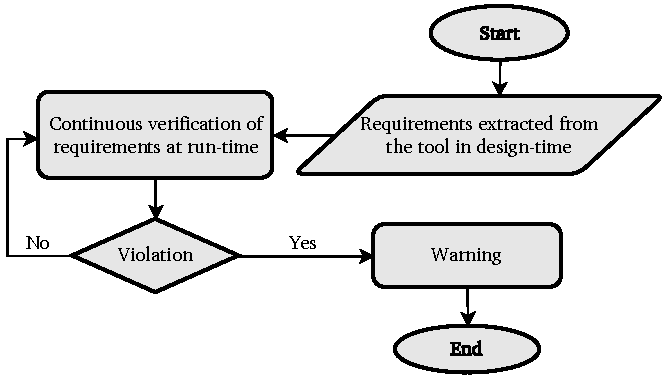
\includegraphics[width=0.8\columnwidth]{figures/monitoring_fc.pdf}
    \caption{The Monitoring mechanism flow chart.}
    \label{fig77}
    \end{figure}
    
    \item \textbf{Task synchronization}: 
    The precision time protocol (PTP) was employed to synchronize the system clocks of multiple nodes. Leveraging the inherent PTP hardware support across all utilized devices, a master clock offset value of approximately 100 ns was attained. Through this synchronization of system time across nodes, the starting time of the simulation can
    be uniformly communicated to all devices, thereby ensuring a synchronized simulation start. Other performance metrics encompassed CPU and RAM utilization, as well as the thermal behavior of the CPU~\cite{correll2005design,askaripoor2023designer}.

    %The Precision Time Protocol (PTP) was used to synchronize the system clocks of multiple nodes. Since all used devices come with PTP hardware support, a master clock offset value of around 100 ns was achieved. With the system time being synchronized among all nodes, the simulation starting time can simply be published to all devices to ensure a synchronized simulation start. Other performance metrics were CPU and RAM utilization as well as thermal development of the CPU.
      \begin{figure}[ht]
    \centering
    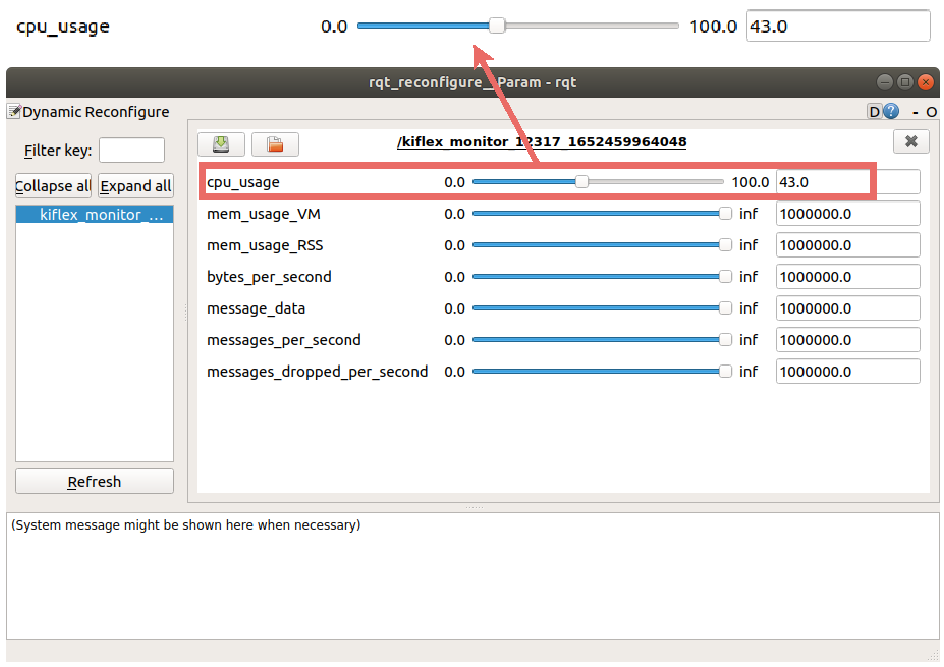
\includegraphics[width=0.95\columnwidth]{figures/GUI_monitoring.pdf}
    \caption{The Monitoring GUI. The threshold values for each specified requirement can be chosen. For example, the threshold value of the CPU usage can be defined inside the red rectangle.}
    \label{fig78}
    \end{figure}
    
      \begin{figure}[hb!]
    \centering
    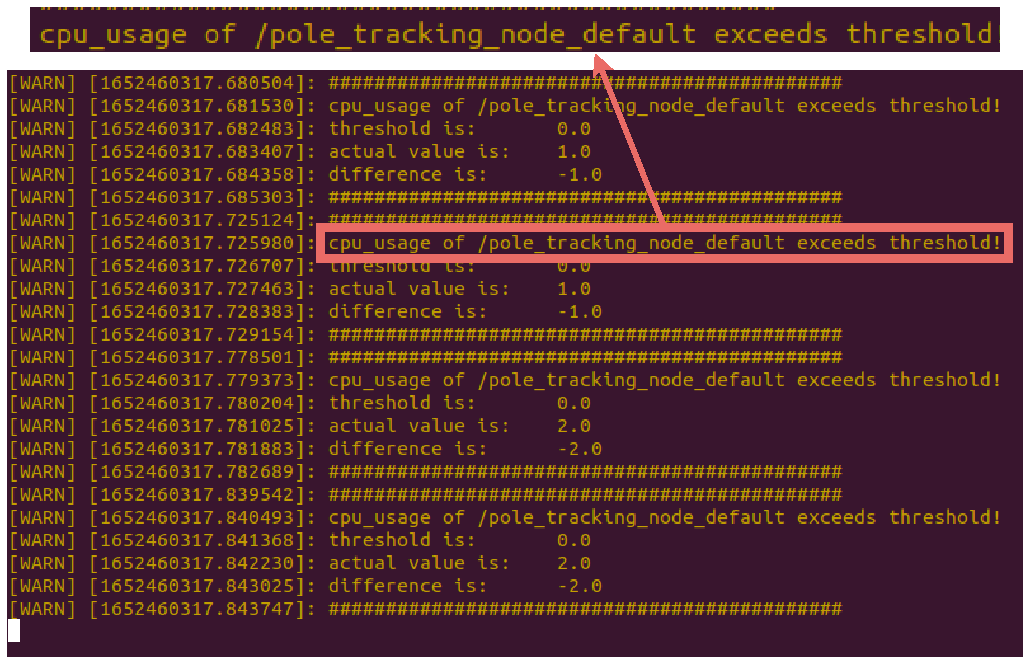
\includegraphics[width=0.9\columnwidth]{figures/result_gui.pdf}
    \caption{The Monitoring GUI. A warning message can be observed in case of violation (red rectangle). }
    \label{fig781}
    \end{figure}
    
    
    \begin{comment}
    \begin{figure}[ht]
    \centering
    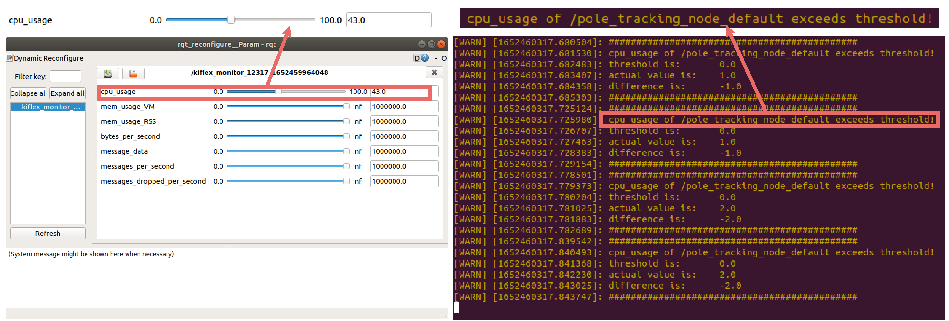
\includegraphics[width=1.1\columnwidth]{figures/monitoring.pdf}
    \caption{A warning message can be observed in case of violation.}
    \label{fig78}
    \end{figure}
    \end{comment}

    
    \item \textbf{Monitoring Mechanism}: 
    %As far as the run-time behavior of the operating system, and middleware in the hardware platform is uncertain due to event-based activities (e.g., application service discovery, and other dynamic and interacting processes causing non-deterministic system resource usage), consideration and creation of the relevant constraints at the design-time by the \textit{E/E Designer} are unrealistic. To establish the verification of the requirements at run-time after deploying the solution, computed by the \textit{E/E Designer}, to the hardware platform,    a monitoring mechanism was developed (See Figure. \ref{fig1}).  
    %To proceed with this mechanism, the approach described in~\cite{askaripoor2021flexible} is followed. The approach has introduced a monitoring mechanism for identifying the timing violations in autonomous driving platforms. As illustrated in the flow chart presented in figure~\ref{fig77}, to mitigate the risk in case of violation of requirements, the monitoring module receives the predefined requirements as given to the tool. It also acquires the run-time values from the hardware platform. In the next step, the design-time requirements and run-time status regarding the requirements are compared and continuously verified. In addition, if any violation occurs, a warning is published so that it announces the violated requirement. 
    As for the run-time behavior of the operating system and middleware within the hardware platform, uncertainty arises due to event-based activities, such as application service discovery and other dynamic, interacting processes that lead to non-deterministic utilization of system resources. Given this complexity, creating and considering pertinent constraints at the design stage by the presented tool becomes impractical.
    In order to establish the validation of requirements, e.g., timing requirements, during run-time after the deployment of solutions computed by the introduced framework onto the hardware platform, a monitoring mechanism has been developed.
    The methodology outlined in~\cite{askaripoor2021flexible} is followed to execute this mechanism. This approach introduces a monitoring mechanism for identifying timing violations in autonomous driving platforms. 
          
    \begin{figure}[b!]
    \centering
    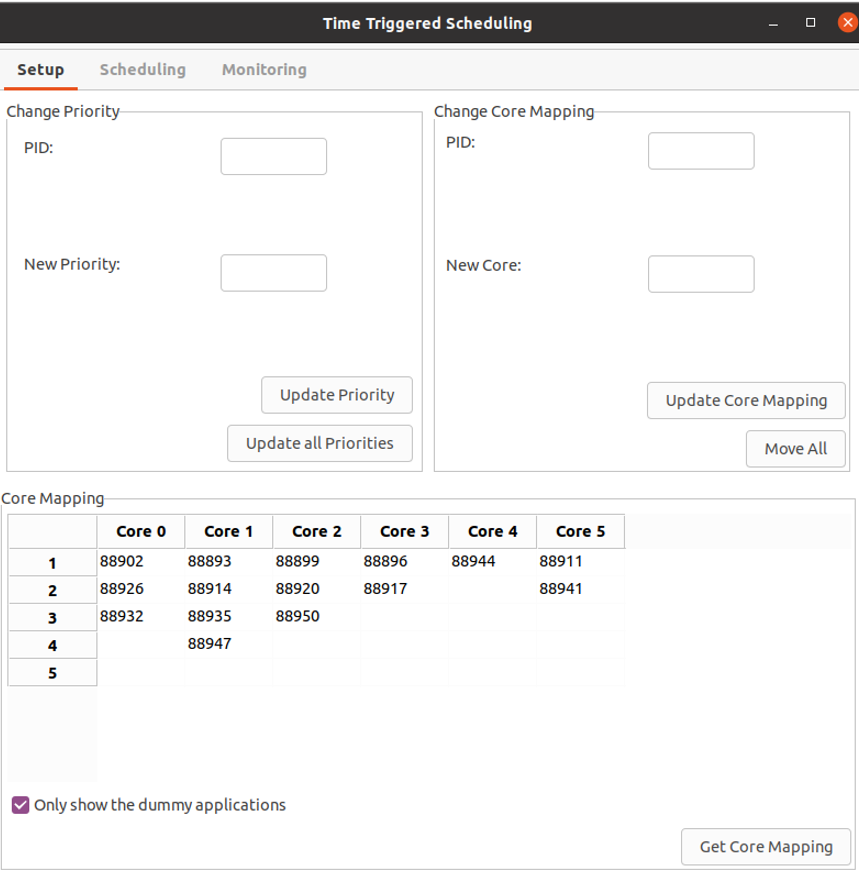
\includegraphics[width=0.8\columnwidth]{figures/gui_scheduling.png}
    \caption{The primary GUI including all features.
    Users can select the priority and assignment for each task on the window.}
    \label{fig79}
    \end{figure}
    The flow chart, depicted in Figure~\ref{fig77}, illustrates the steps involved. To mitigate risks arising from requirement violations, the monitoring module receives the predefined requirements initially given to the tool. Concurrently, it collects real-time values from the hardware platform. In the subsequent phase, a continuous comparison and verification process is initiated between the design-time requirements and the real-time status concerning these requirements. Furthermore, if any violation occurs, an alert is issued to announce the breached requirement, as illustrated in Figure~\ref{fig77}~\cite{9613692}. Figure~\ref{fig78} shows the graphical user interface (GUI) for the integrated monitoring mechanism as part of the main GUI.
    Within this interface, the option to establish a threshold value for each requirement is presented, exemplified by CPU usage, as depicted in Figure~\ref{fig78}. 
    %where a threshold value can be specified for each requirement, e.g., CPU usage, as shown on the left side of figure~\ref{78}.
    Furthermore, in instances where the value of any requirement surpasses the determined threshold, an immediate warning message is generated, as demonstrated based on Figure~\ref{fig781}~\cite{askaripoor2021flexible,9613692, askaripoor2023designer}.

    The monitoring mechanism is a substantial part of the performance evaluation as the measuring must be very accurate but also very light-weight to not influence the measured metrics~\cite{askaripoor2021flexible,9613692, askaripoor2023designer}. %The main performance metric in the current run-time evaluation was the start and stop time of each task. From that, one can calculate the start and stop jitter, i.e. the difference between the actual and expected start and stop times. Start and stop times were measured by tracing the system calls indicating a change in process state using strace.
    The primary performance metric during the ongoing run-time evaluation pertained to each task's initiation and cessation times. This specific metric allowed for the computation of both start and stop jitter, representing the variance between the actual and expected start and stop times. The determination of start and stop times was facilitated through a meticulous tracing of system calls that signified transitions in process states, a process efficiently carried out using\textit{strace}. Other performance metrics included CPU and RAM utilization, as well as the thermal development of the CPU, which are discussed in the following. 
    
    %As an example, a safety-critical application, \emph{A}, must be isolated as well as mapped on a CPU core, \emph{C}, which meets the ASIL D based on HW properties.

    \begin{figure}[t]
    \centering
    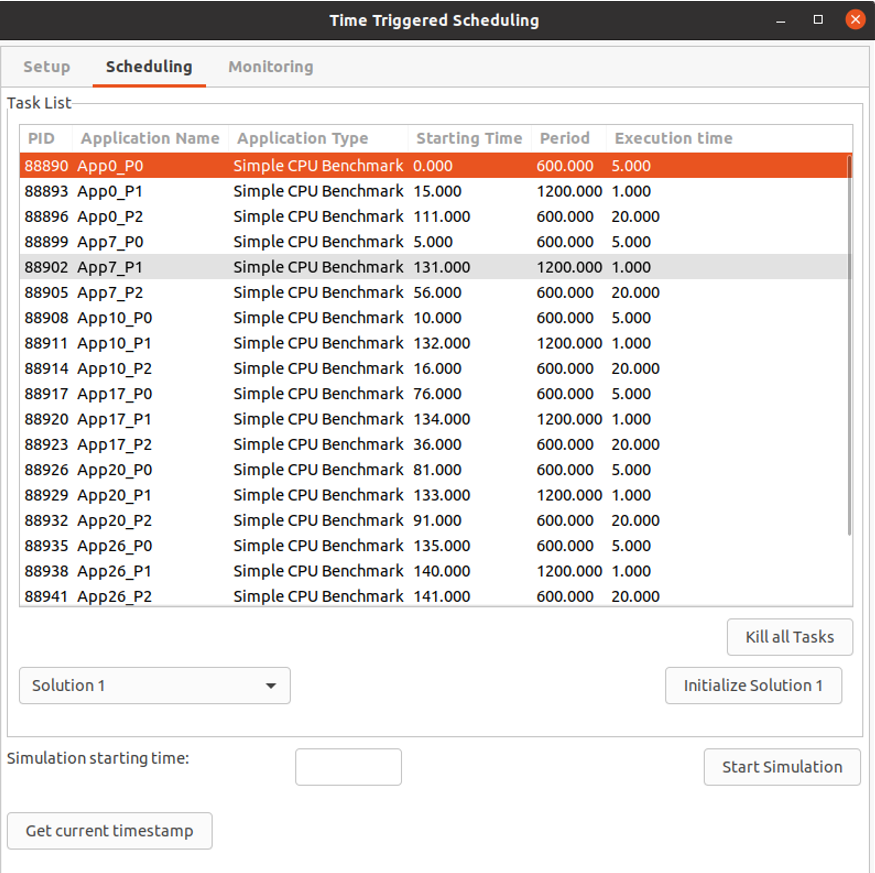
\includegraphics[width=0.8\columnwidth]{figures/TTScheduling.png}
    \caption{The primary GUI including all features. The window visually represents the priority, period, and execution time associated with each task.}
    \label{fig0079}
    \end{figure}
    
    \begin{comment}
    \begin{figure}[ht]
    \centering
    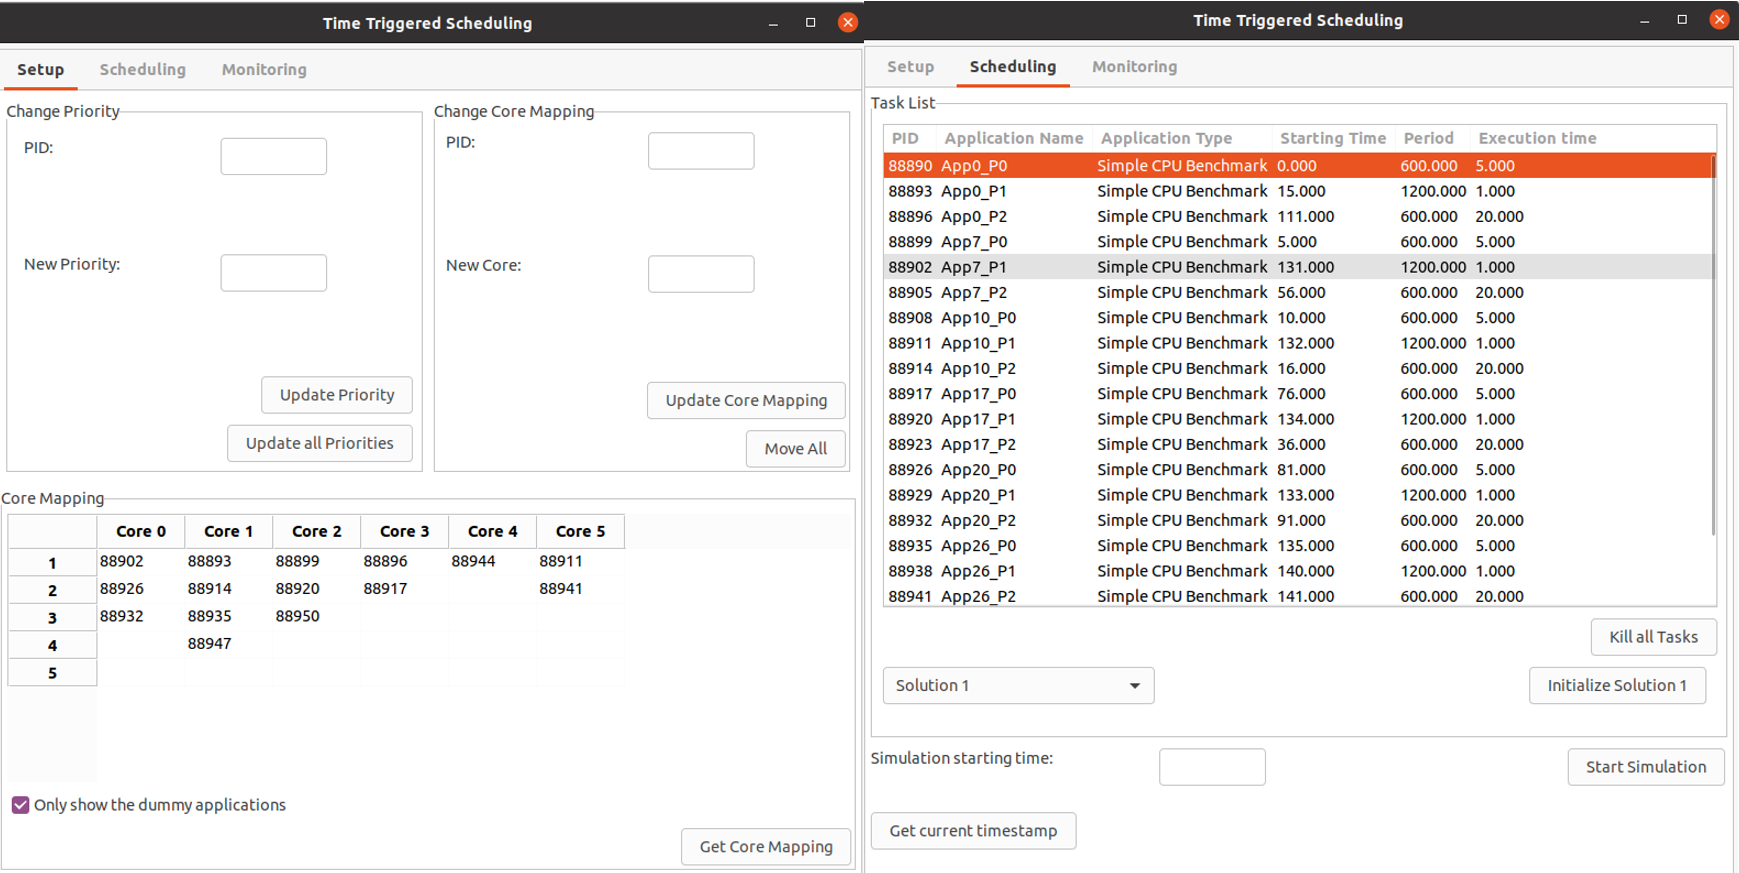
\includegraphics[width=1\columnwidth]{figures/gui.png}
    \caption{The primary GUI including all features.
    On the left-hand side, users can select the priority and assignment for each task. The window on the right provides a visual representation of the priority, period, and execution time associated with each task.}
    \label{fig79}
    \end{figure}
    \end{comment}

    %After taking this requirement into account in the constraints system of the \textit{E/E Designer}, it is deployed to the \textit{AHPCC} for a real-world scenario. Therefore, the \textit{Monitoring System} verifies in real-time whether application \emph{A} has been isolated and assigned to core \emph{C} or not. This observation is visualized as a warning in a graphical user interface (GUI) in case of violation (See Figure. \ref{fig4}). In addition, the \textit{Monitoring System} evaluates the \textit{E/E Designer} performance in terms of various metrics on account of utilizing its mapping solution and a random mapping for the \textit{AHPCC}. This system also checks the possible safety violations created by an unpredictable operating system and middleware procedures such as multi-threading, automatic resource allocation, etc (See Figure. \ref{fig1}). 
    
    
    
    
    
    
    \item \textbf{GUI}: 
         A user-friendly graphical interface has been developed to facilitate the deployment of the calculated solutions. This interface seamlessly integrates all the functionalities described above into a single program. This integration enables the automated deployment of mapping and communication solutions onto the hardware, simplifying the process of replicating experiments. Moreover, the developed GUI assumes the role of initiating the monitoring procedures. It adeptly manages the collection and processing of the measured data, a process elucidated in the finer details of the monitoring mechanism. This cohesive integration ensures a seamless and efficient flow of tasks, enhancing the overall user experience and research methodology~\cite{askaripoor2023designer, askaripoor2021flexible}. Figure~\ref{fig79} illustrates the GUI configuration for deploying the mapping and time-triggered scheduling solutions on the hardware platform.
         For example, based on Figure~\ref{fig79}, the priority of each task and its allocation to a specific core can be managed. In Figure~\ref{fig0079}, the designated period and execution time of each task, along with its name and priority, are presented.
    %For example on the left, the priority of each task as well as its assignment to a specific core can be handled. On the right side, the defined period and execution time of each task  as well as its name and priority can be seen.
    
    
    %To facilitate the deployment of calculated solutions, a graphical user interface has been developed that integrated all the above-described functionalities into one program. By that, mapping and communication solutions can automatically be deployed onto the hardware to easily repeat the experiments. Furthermore, the developed GUI starts the monitoring and takes care of gathering and processing the measured data, as explained in the monitoring mechanism details.
    \end{itemize}





 





%Each task is modeled as a Linux process of a custom benchmark application. The benchmark calculates ten digits of pi using the Gauss–Legendre algorithm in an infinite loop and is thus CPU-bound. Besides, there are sender and receiver applications that support TCP-based message transfer.

%\paragraph{Scheduling and Dispatching} The scheduling is simulated by another standard Linux process that is assigned the highest real-time priority 99. It is implemented using a C timer function that invokes a callback every 1000 nanoseconds to check if a task should be scheduled or stopped at that specific timestamp. Before the simulation starts, the number of hyperperiods must be specified so that the start and stop times for every task can be calculated in advance and stored in a sorted array. Therefore, in the timer callback, it is only necessary to compare the current counter value with the top entry of the aforementioned array, thus reducing the invocation time of the callback to a minimum. When a task must be started or stopped, the scheduler will send a POSIX signal to the corresponding task. The task is stopped using the SIGKILL signal and restarted using the SIGCONT signal.

%\paragraph{Task mapping} The tasks are mapped to specific cores before the start of the simulation. For that, their CPU affinity is set using the taskset command, which will cause the Linux scheduler to bond the process to a given CPU core. To ensure that the tasks are not interrupted by any other processes running on the system, each task is assigned the second-highest real-time priority of 98. By that, the tasks are prioritized over every other process by the Linux scheduler but can still be interrupted by the simulation scheduler. Furthermore, all other systems and extraneous processes are mapped to CPU core 0, except bounded kernel threads, to isolate the simulated cores.

    %\paragraph{Task synchronization} The Precision Time Protocol (PTP) was used to synchronize the system clocks of multiple nodes. Since all used devices come with PTP hardware support, a master clock offset value of around 100 ns was achieved.With the system time being synchronized among all nodes, the simulation starting time can simply be published to all devices to ensure a synchronized simulation start.Other performance metrics were CPU and RAM utilization as well as thermal development of the CPU.
    %\paragraph{Monitoring} Monitoring is a substantial part of the performance evaluation as the measuring must be very accurate, but also very light-weight to not influence the measured metrics~\cite{askaripoor2021flexible,9613692}.







    %%%%%%%%%%%%%%%%%%%%%%%%%%%%%%%%%%%%comment%%%%%%%%%%%%%%%%%%%%%%%%%%%%%%%%%%
    \begin{comment}
    \begin{figure*}[t]
	\centering
	%\begin{adjustbox}{minipage=19.5cm, center}
		\makebox[\textwidth][c]{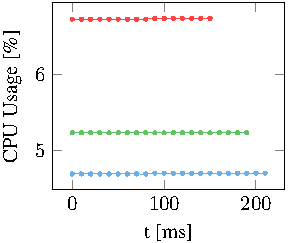
\includegraphics[width=0.4\textwidth]{figures/CPU_Usage.pdf}}
	%\end{adjustbox}
	\caption{Comparison of different metrics. Red is the time-triggered scheduling, blue is FIFO scheduling, and green is Round Robin scheduling}
	\label{fig:metrics}
    \end{figure*}
    \begin{figure*}[ht]%
	\centering
	\subfloat[\centering]{{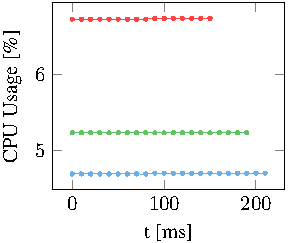
\includegraphics[width=7cm]{figures/CPU_Usage.pdf} }}%
	\qquad
	\subfloat[\centering]{{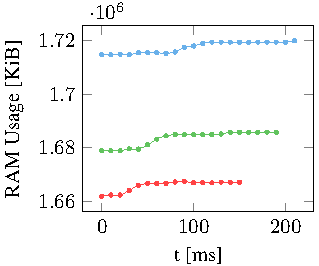
\includegraphics[width=7.51cm]{figures/ram_usage.pdf} }}%
	\qquad
	\subfloat[\centering]{{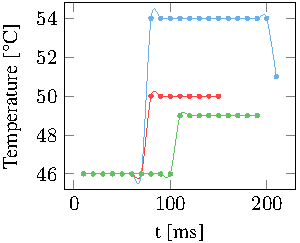
\includegraphics[width=7cm]{figures/temp.pdf} }}%
	
	\caption{Comparison of different metrics. Red is the time-triggered scheduling, blue is FIFO scheduling, and green is Round Robin scheduling.}%
	\label{fig8_side}%
	
	\end{figure*}
    \end{comment}
   %%%%%%%%%%%%%%%%%%%%%%%%%%%%%%%%%%%%comment%%%%%%%%%%%%%%%%%%%%%%%%%%%%%%%%%%











%The main performance metric was the start and stop time of each task. From that, one can calculate the start and stop jitter, i.e. the difference between the actual and expected start and stop times. Start and stop times were measured by tracing the system calls indicating a change in process state using strace.


%\paragraph{GUI} To facilitate the deployment of calculated solutions, a graphical user interface has been developed that integrated all the above-described functionalities into one program. By that, mapping and communication solutions can automatically be deployed onto the hardware to easily repeat the experiments. Furthermore, the developed GUI starts the monitoring and takes care of gathering and processing the measured data.

%\section{Experimental Setup}
%\label{sec:setup}




%\subsection{Software}
%Isolating different applications from another using partitioning requires a hypervisor. There are a few open-source hypervisors available mostly for specialized guest and host CPU architectures and use cases. The most common ones are Xen and KVM. Unlike other open-source virtualization solutions, both are well maintained and run on ARM processors and Unix-based systems.\paragraph{Xen}\label{sec:xen}

%Xen \cite{Xen2021} is a type-1 hypervisor that was originally developed at the University of Cambridge but is now maintained by the Linux Foundation. Many commercial and open-source virtualization projects use Xen as a basis. In the Xen Project, a running instance of a partition is called a domain. Xen runs directly on the hardware and is loaded by the bootloader. The Xen hypervisor requires a special partition called domain 0 (dom0) to be running which is initialized after the start of the hypervisor. Dom0 has more privileges than the other partitions and is used for administrative tasks like starting new domains. Also, dom0 can access the hardware directly and contains the device drivers.

%Xen is the only pure type-1 hypervisor available as an open-source project. Besides, it has other benefits like operating system agnosticism or paravirtualization. However, without the documentation on customizing the PDK, for example, to change the boot sequence, it is not possible to install Xen hypervisor on an Nvidia Drive with any reasonable amount of resources.\paragraph{KVM}\label{sec:kvm}

%Kernel-based Virtual Machine (KVM) \cite{KVM2016} is a virtualization module that can be integrated into a Linux kernel and turns it into a hypervisor. Therefore, KVM can be installed on an Nvidia Drive without modifying the firmware. The Linux kernel then provides all necessary features like scheduling, memory management, and drivers; the other partitions are standard Linux processes. It also requires a modified QEMU version to emulate hardware. KVM can neither be distinctly considered type-1 nor type-2.KVM was installed on an Nvidia Drive running DRIVE OS 5.2. To evaluate the performance of the KVM hypervisor on the Nvidia Drive, one partition with Ubuntu Server 18.04 was set up.\subsection{Hardware}
 

    \subsubsection{Mapping evaluation}
    %The mapping evaluation was based on 40 applications, each consisting of three threads. Their periods and execution times can be found in Table \ref{table:threads}. Therefore, there are in total 120 threads which are mapped onto different cores. The time-triggered scheduling was evaluated against FIFO and Round Robin with a time quantum of 1 ms, which was selected based on the shortest execution time. Since the execution of all cores is independent of one another, and the workload is distributed approximately equally among all cores in the evaluated solution, we will only look at the results measured on one core to conclude the overall performance.
        
          \begin{table}[t!]
	\begin{center}
		\caption{Periods and execution times of threads for each sample application.}
		\begin{tabular}{@{}ccc@{}}
			\toprule
			Name & $t.p$ (Period) [ms] & $t.e$ (Execution time) [ms]\\
			\midrule
			$T_{0}$ & 600 & 5 \\
			$T_{1}$ & 1200 & 1 \\
			$T_{2}$ & 600 & 20 \\
			\bottomrule
		\end{tabular}
		 \label{threads}
	\end{center}
    \end{table}
    The mapping evaluation was based on 40 applications, each consisting of three threads. The periods and execution times of these threads can be found in Table~\ref{threads}. A total of 120 application threads are mapped onto different cores. The time-triggered scheduling was evaluated against first in, first out (FIFO) and Round Robin with a time quantum of 1 ms, which was selected based on the shortest execution time~\cite{askaripoor2023designer,leontyev2007tardiness, rasmussen2008round}.
         \begin{figure}[b!]
	\centering
	%\begin{adjustbox}{minipage=22cm, center}
		\makebox[\textwidth][c]{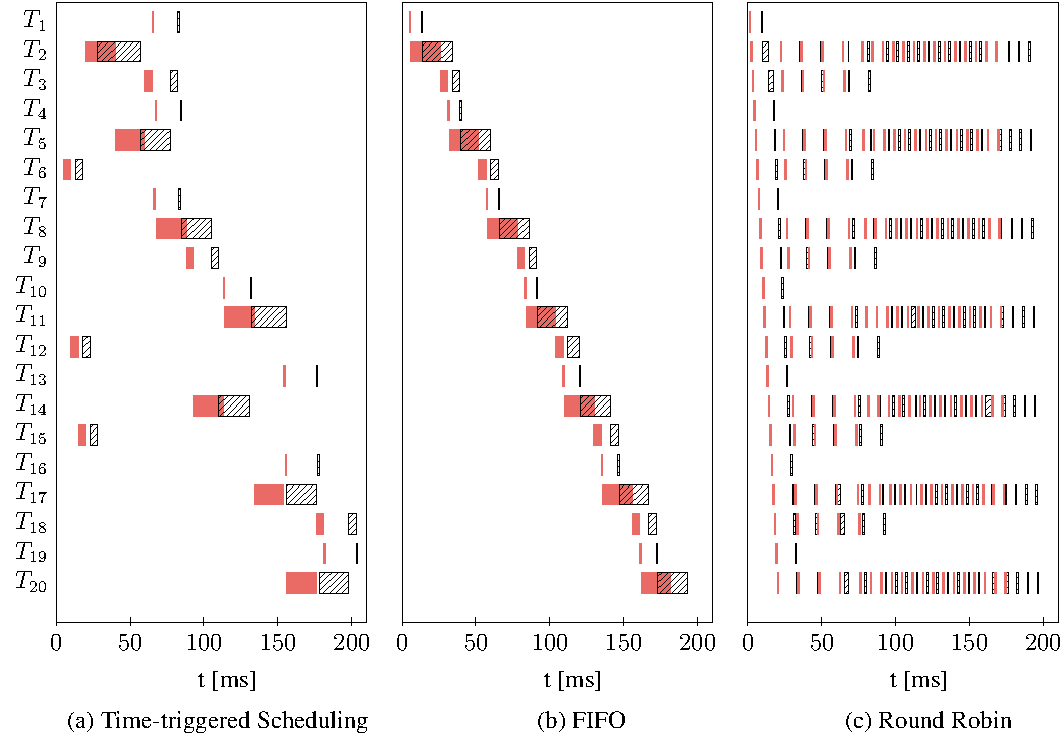
\includegraphics[width=1\textwidth]{figures/gantt_v3.pdf}}
	%\end{adjustbox}
	\caption{Gantt charts of the different scheduling solutions for CPU 5. The
    red bars represent the planned execution, while the hatched bars stand for the actual execution~\cite{askaripoor2023designer}.}
	\label{fig:gantt}
    \end{figure}
    FIFO scheduling is a simple and intuitive scheduling algorithm that operates on a first-come, first-served basis. In this approach, the process that arrives first is executed first, and subsequent processes are executed in the order of their arrival~\cite{leontyev2007tardiness}. In comparison, Round Robin scheduling is a preemptive scheduling algorithm that allocates a fixed time quantum to each process in a cyclic manner. It ensures fairness by allowing each process to execute for a predefined time slice or quantum before moving to the next process. If a process does not complete its execution within the time quantum, it is temporarily suspended, and the next process in the queue is allowed to run. The suspended process is then placed back in the ready queue, and execution resumes from where it left off during the next scheduling cycle~\cite{rasmussen2008round}.
 

       \begin{figure}[t!]
	\centering
	\makebox[\textwidth][c]{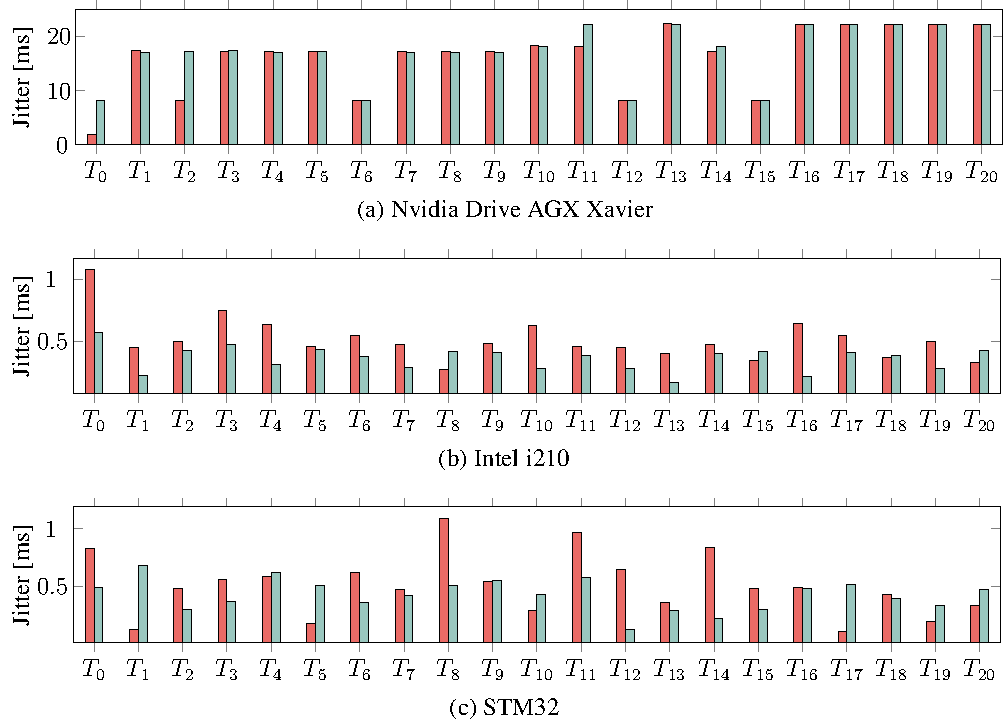
\includegraphics[width=1\textwidth]{figures/jitter_v2.pdf}}
	\caption{Start and stop jitters of each thread measured for the time-triggered scheduling over one hyperperiod. These are the measurements on CPU core 5. Red bars represent the start jitter, and the green bars the stop jitter~\cite{askaripoor2023designer}.}
	\label{fig:jitter}
    \end{figure}
    Given that the execution of all cores operates independently from each other and the workload is distributed relatively evenly across all cores in the assessed solution, for the sake of illustration, only the results from one core are presented. This is due to the similarity in behavior demonstrated by the other cores.

     %Since the execution of all cores is independent of one another and the workload is distributed approximately equally among all cores in the evaluated solution, for illustration purpose, only results on one core is shown, as other cores demonstrate similar behavior.

    %Since the execution of all cores is independent of one another and the workload is distributed approximately equally among all cores in the evaluated solution, for illustration purpose, only results on one core is shown, as other cores demonstrate similar behavior.

    
    
    
    
    Figure~\ref{fig:gantt} depicts the expected and actual start and stop times for the three evaluated scheduling policies. It is noticeable that across all setups, there are cases where threads commence even after the expected stop time. This tendency is more pronounced with shorter execution times, making it especially notable in the Round Robin configuration.


    %figure~\ref{fig:gantt} shows the expected and actual starting and stop times for the three tested scheduling policies. It can be seen that in all configurations, there are threads that started even after the expected stop time. This is particularly true for shorter execution times and therefore especially predominant in the Round Robin setup.

    \begin{figure}[t!]
	\centering
	%\begin{adjustbox}{minipage=19.5cm, center}
		\makebox[\textwidth][c]{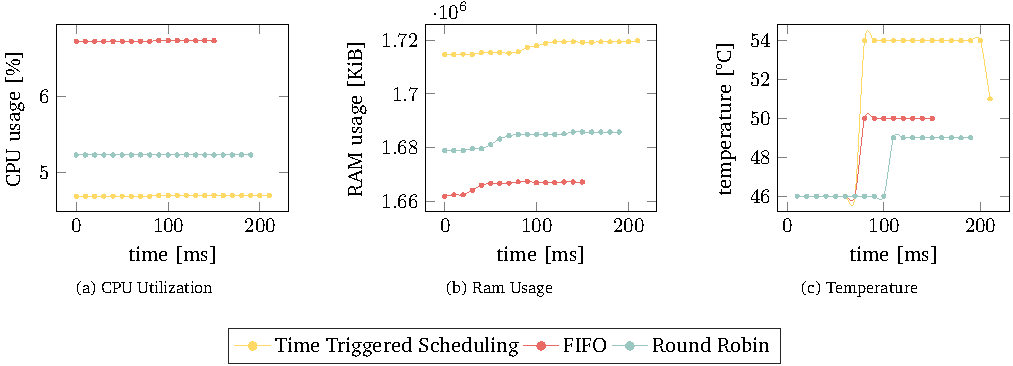
\includegraphics[width=1\textwidth]{figures/metrics_analysis.pdf}}
	%\end{adjustbox}
	\caption{Comparison of different metrics. Yellow is the time-triggered scheduling, red is FIFO scheduling, and green is Round Robin scheduling~\cite{askaripoor2023designer}.}
	\label{fig:metrics}
    \end{figure}
    
     Figure~\ref{fig:jitter} shows the jitter measurements for time-triggered scheduling across various hardware platforms, namely Nvidia Drive AGX Xavier, Intel i210 development kit, and STM development kit~\cite{Intel, STM, NVIDIA}. The observation reveals a noteworthy disparity in jitter generation. Particularly, the Nvidia Drive exhibits a notable level of jitter. The average jitter on the Nvidia Drive surpasses that on the Intel i210 by a factor of approximately 36.6, despite both setups being the same~\cite{askaripoor2023designer}.

    %figure~\ref{fig:jitter} shows the jitter measurements for time-triggered scheduling on all the hardware platforms including Nvidia AGX Drive, Intel i210 development kit, and STM development kit. It can be seen that the jitter produced on the Nvidia Drive is generally significant. The average jitter is approximately 36.6 times higher on the Nvidia Drive compared to the Intel i210 for the same setup.
    %\vspace{10pt}
 
    %The primary reason is that the jitter produced on the Nvidia Drive is generally very significant. This is illustrated by the fact that the average jitter is around 36.6 times higher on the Nvidia Drive compared to the Intel i210 for the same setup. figure~\ref{fig:jitter} depicts the jitter measurements for the time-triggered scheduling on both hardware platforms.
      
     \begin{figure}[ht]
	\centering
	\makebox[\textwidth][c]{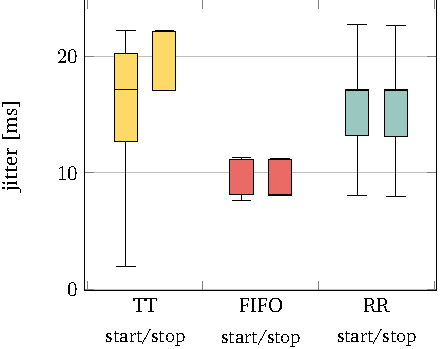
\includegraphics[width=0.5\textwidth]{figures/jitter_box.pdf}}
	\caption{Spread of start and stop jitter for the tested scheduling policies. The box plot shows the minimum and maximum values, the lower and upper quantiles, and the mean. The yellow, red, and green boxes represent results for time-triggered, FIFO, and Round Robin scheduling schemes, respectively.}
	\label{fig:jitter_boxplot}
    \end{figure}
    
        The results of the CPU, RAM, and temperature measurements are illustrated in Figure~\ref{fig:metrics}. While there are observable distinctions among all the setups, they are not deemed significant. Moreover, none of the scheduling schemes exhibits superior performance across all metrics.

        Furthermore, the offset between the actual and expected execution times remains comparatively constant with FIFO scheduling. This can also be seen by looking at Figure~\ref{fig:jitter_boxplot}, which shows that the jitter is much more predictable for FIFO than for the time-triggered scheduling solution. This indicates that the jitter produced by the dispatcher is centered around a constant value with a low spread.
        Nevertheless, all threads finished within their specified period, and no deadline violation occurred in any of the tested setups~\cite{askaripoor2023designer}.

         %The results of the CPU, RAM, and temperature measurements are depicted in figure~\ref{fig:metrics}. There are noticeable but not significant differences among all the setups. Also, none of the scheduling schemes outperforms the others in all metrics.

    
    
    
%%%%%%%%%%%%%%%%%%%%%
%% Metrics
%%%%%%%%%%%%%%%%%%%%%




%%%%%%
%% Gantt
%%%%%%



%%%%
% Jitter
%%%%



%%%%%%%%%
% Jitter Boxplot
%%%%%%%%%



    
    \subsubsection{Communication evaluation} 
    Apart from the mapping evaluation, a communication assessment was performed where an E/E architecture is modeled using the introduced computer-aided tool, and its provided solution is deployed on an actual hardware setup with the same topology designed by the tool. The solution consists of schedules for application threads executing on each ECU, as a sender and receiver, and for communication tasks routing over each link. The multi-objective optimization comprising end-to-end latency and response time was applied to the solution.   
    This experiment measured the end-to-end latency and response time for communication messages~\cite{askaripoor2023designer}. 
    
     \begin{figure}[ht]
	\centering
	\makebox[\textwidth][c]{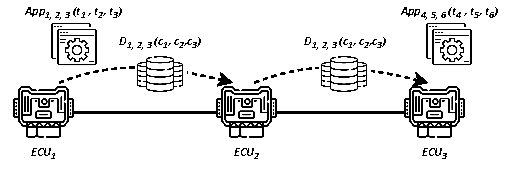
\includegraphics[width=0.9\textwidth]{figures/Communication_setup_topology.pdf}}
	\caption{Topology of the tested communication setup. Threads 1-3 on $ECU_1$  each send a communication packet to threads 4-6 on $ ECU_3 $. All three packets ($c_1, c_2, c_3$) are routed over $ECU_2$~\cite{askaripoor2023designer}.}
	\label{fig:communication_topology}
    \end{figure}
    
    Communication was tested using a scenario consisting of three connected nodes: an Nvidia TX2 Developer kit (\textit{ECU$_1$}), the Nvidia Drive AGX Xavier (\textit{ECU$_2$}), and an Intel i210 Developer kit (\textit{ECU$_3$}) based on Figure~\ref{fig:communication_topology}. On\textit{ ECU$_1 $ } ran three applications, each comprising a thread, each of those sending a communication packet to a respective receiver task on \textit{ECU$_3$} via \textit{ECU$_2$}. Figure~\ref{fig:communication_topology} visualizes the setup. As mentioned earlier, the end-to-end latencies and response times of the three communication messages, each including a communication task defined above, are measured~\cite{askaripoor2023designer}.




    \begin{table}[ht]
	\begin{center}
		\caption{Communication solution calculated by the presented framework.}
		\begin{tabular}{@{}lcc@{}}
			\toprule
			Name & Start time [µs] & Stop time [µs] \\
			\midrule
			$t_1.st$ & 0.00 & 90.00 \\
			$t_2.st$ & 90.00 & 290.00 \\
			$t_3.st$ & 290.00 & 440.00 \\
			\midrule
			$c_1.st^{l_{1}}$ & 100.0 & 112.60 \\
			$c_2.st^{l_{1}}$ & 300.00 & 312.60 \\
			$c_3.st^{l_{1}}$ & 450.00 & 462.00 \\
			\midrule
			$c_1.st^{l_{2}}$ & 127.60 & 140.20 \\
			$c_2.st^{l_{2}}$ & 327.60 & 340.20 \\
			$c_3.st^{l_{2}}$ & 477.60 & 490.20 \\
			\midrule
	    	$t_4.st$ & 150.20 & 250.20 \\
			$t_5.st$ & 650.20 & 850.20 \\
			$t_6.st$ & 500.20 & 650.20 \\
			\bottomrule
		\end{tabular}
		\label{table:communication1}
	\end{center}
    \end{table}
    

    The communication links had a theoretical bandwidth of 1000 Mbit/s; however, 940 Mbit/s were measured when also running PTP synchronization over the same links.
    The size of the communication messages was chosen to fit into one single Ethernet frame of 1500~B size. Therefore, the frame length of each communication task was set to 12.6 µs.
    The solution calculated by the proposed tool is presented in Table~\ref{table:communication1}. It shows the start and stop times for the sender and receiver applications and the communication tasks over one hyperperiod~\cite{askaripoor2023designer}.


     \begin{figure}[ht]
	\centering
	\makebox[\textwidth][c]{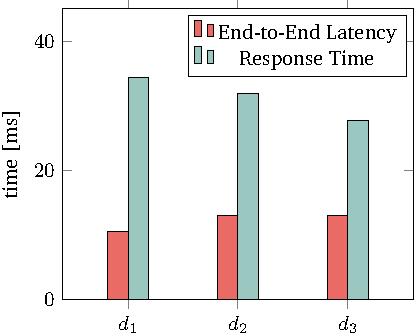
\includegraphics[width=0.5\textwidth]{figures/ee_latency_setup.pdf}}
	\caption{Measured end-to-end latency and response times of the three communication messages using Nvidia Drive AGX, Nvidia TX2, and Intel i210 developer kits as the setup.}
	\label{fig:end_to_end_latency}
    \end{figure}

    Figure~\ref{fig:end_to_end_latency} shows the results of the experiments. It is noticeable that the measured end-to-end latencies do not vary much but are in the order of 10 ms.
    Even though the actual frame length is considerably smaller than these values, the influence of start and stop jitters in the application threads profoundly impacts the overall latency metrics. This, in turn, led to instances of deadline violations during the communication testing phase~\cite{askaripoor2023designer}. This phenomenon can be attributed to the significant jitter introduced by the Nvidia AGX Drive, vividly illustrated in Figure~\ref{fig:jitter}.
         \begin{figure}[b!]
	\centering
	\makebox[\textwidth][c]{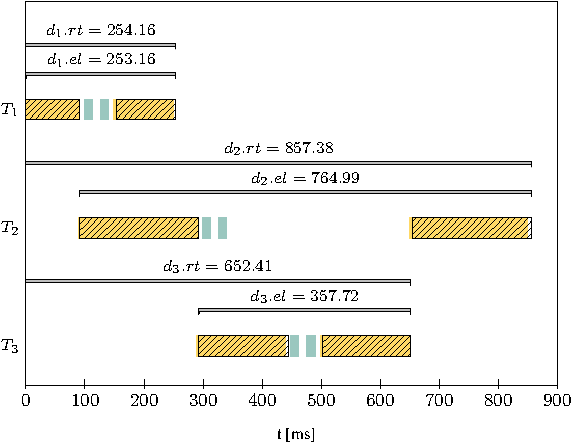
\includegraphics[width=0.85\textwidth]{figures/gantt_communication_v2.pdf}}
	\caption{Results of the communication evaluation experiment using STM development kits. The yellow bars represent the expected execution, while the hatched bars represent the actual execution times of the sender and receiver applications. The green bars indicate the planned schedule of the communication messages. The response time and end-to-end latency of each communication message are also shown~\cite{askaripoor2023designer}.}
	\label{fig:end_to_end_latency1}
    \end{figure}
    %While the actual frame length is significantly smaller compared to these numbers, the start and stop jitters of the application threads heavily influence the overall latencies. As a result, deadline violations occurred during the communication testing. The reason is the significant jitter created by the Nvidia AGX Drive, as presented in figure~\ref{fig:jitter}. 
    
    Due to this effect, a decision was made to execute the communication experiment using STM32-based development boards~\cite{STM}. These boards exhibit a notably lower scheduling jitter, ensuring minimal disruption to the execution of the synthesized communication solution. It is important to note that this particular experiment adhered to the same topology and design-time outcomes, shown in Table~\ref{table:communication1}, as the initial communication experiment, both of which were generated by the tool.
    
    

    
    
    %Therefore, the communication experiment was performed using the STM32-based development boards because their low scheduling jitter has only minimal influence on the execution of the synthesized communication solution. In this experiment, the same topology and design-time results generated by the tool as the first communication experiment were utilized. 
    The CAN configuration was chosen as the communication protocol between ECUs in this setup. This choice stems from its widespread usage within the automotive domain and its comparative simplicity when contrasted with other protocols regarding the essential hardware setup and software implementation, as described in Chapter~\ref{basicConcepts}. Moreover, it has relatively little overhead and thus simplifies the calculations.
    %In this setup, the CAN configuration was selected as the communication protocol between ECUs since it is a very common protocol in the automotive domain and is simple compared to other protocols in terms of required hardware setup and software realization, as described in the Chapter~\ref{basicConcepts}. In addition, it has relatively little overhead and thus simplifies the calculations.
    The communication links had a theoretical bandwidth of 11,520 bytes/s, which is a common baud rate. The size of the communication messages was chosen to be 145 bytes, deliberately kept small to fit into a single frame and avoid fragmentation and long verification times that can potentially influence the results. Each communication task's frame length was set to 12.6 ms, calculated by dividing the size of the communication message by the bandwidth. The interpacket gap was set to 10 ms. The user can specify these communication properties for each network protocol in the framework, similar to how timing parameters can be determined in the framework's frontend.
    %The solution calculated by the \textit{E/E Designer} is presented in the right section of Table~\ref{threads}. It shows the start and stop times for the sender and receiver application threads, as well as for the communication tasks, over one hyperperiod.




    %STM32-based development boards were used for the communication experiments because their low scheduling jitter has only minimal influence on the execution of the synthesized communication solution.
    %The communication links had a theoretical bandwidth of 11,520 bytes/s, which is a common baud rate. The size of the communication messages was chosen to be 145 bytes, deliberately kept small to fit into a single frame and avoid fragmentation and long verification times that could potentially influence the results. Each communication task's frame length was set to 12.6 ms, calculated by dividing the size of the communication message by the bandwidth.
    %The interpacket gap was set to 10 ms. These communication properties can be specified by the user for each network protocol in the framework, similar to how timing parameters can be determined in the frontend. The solution calculated by the \textit{E/E Designer} is presented in the right section of Table~\ref{threads}. It shows the start and stop times for the sender and receiver application threads, as well as for the communication tasks, over one hyperperiod.



    Figure~\ref{fig:end_to_end_latency1} shows the results of the communication experiments using the STM boards. It can be seen that the measured response times and end-to-end latencies for all three communication messages, $d_1$, $d_2$, and $d_3$, closely align with the anticipated values, indicating the absence of any deadline violations.

    %the measured response-times and end-to-end latencies are very close to the expected values and hence there is no deadline violation.



    \section{Quantitative and Qualitative Evaluation}\label{qualTime}

    %In order to evaluate the performance, usability and practicability of the E/E Designer, several use cases are solved and multiple experts are interviewed.The following subsections provide a detailed overview of the quantitative and qualitative results.
    To evaluate the performance, usability, and practicality of the illustrated model-based tool, a series of use cases were addressed through both manual and automated approaches. The following subsections provide a detailed analysis of the findings, encompassing both quantitative and qualitative aspects.









    \subsection{Quantitative Analysis of Various Case Studies}
        
    %For the quantitative evaluation of the proposed framework, various mapping and mapping \& routing use cases are solved, once manually and once using the E/E Designer tool.
    For the quantitative evaluation of the proposed framework, a series of mapping and mapping \& routing use cases are undertaken. These cases are addressed through two distinct approaches: manual solution and utilization of the E/E Designer tool.




    
    
    \subsubsection{Mapping Case Studies}
    
    %Mapping use cases focus only on the correct assignment of applications to the different ECUs and calculation of schedules for the application threads, but do not include message routing and communication tasks scheduling. For the evaluation, the following use cases are created:
    
    The mapping use cases center solely on accurately assigning applications to diverse ECUs and determining schedules for the application threads. However, these use cases do not encompass aspects such as message routing and scheduling communication tasks. To facilitate the evaluation process, the ensuing use cases have been established. The following case studies are given to a group of students to execute the quantitative and qualitative analysis utilizing manual and tool-assisted approaches.
    
    \begin{itemize}
    \item M\_1 :4 ECUs, 4 applications 
    \item M\_2: 6 ECUs, 8 applications 
    \item M\_3: 8 ECUs, 12 applications
    \item M\_4: 8 ECUs, 18 applications 
    \item M\_5: 8 ECUs, 24 applications
    \item M\_6: 8 ECUs, 32 applications. 
    \end{itemize}
    Note that each application consists of two threads within the above-mentioned use cases.
    To address these use cases, the following constraints are taken into consideration.    \begin{itemize}
        \item Time-triggered scheduling constraints for application threads. This ensures the feasibility of application execution
        \item Each ECU must execute at least one application
    \end{itemize}
    
    %\textbf{Evaluation}
     %figure~\ref{mapping_use_cases_setup_time}~(a) shows the time for modeling/designing each above-mentioned use case using manual and the proposed framework approaches. As it can be seen for small size topologies, the overhead of the E/E designer causes a slightly longer configuration time. As soon as the size becomes bigger, and especially if the case study comprises multiple objects having the same properties, a relevant speedup can be achieved. This speedup is mainly related to the feature of automatic creation of SW/HW components explained in the Chapter~\ref{frontend} which brings the possibility of creating multiple elements at once.
     
     Figure~\ref{mapping_use_cases_setup_time}~(a) illustrates the time required for modeling and designing each of the use cases, as discussed earlier, employing both the manual and proposed framework approaches. Notably, for smaller topology sizes, the proposed model-based framework introduces a slight overhead that leads to a marginally extended configuration time. However, as the topology size scales up, particularly when the case study encompasses multiple objects sharing similar properties, a discernible acceleration in the process becomes evident.
     This acceleration is closely tied to the intrinsic capability outlined in Chapter~\ref{frontend}, which pertains to the automatic creation of software/hardware components. This feature empowers the simultaneous generation of multiple elements, thereby contributing significantly to the observed speedup.

    \begin{figure}[t]
	\centering
	\makebox[\textwidth][c]{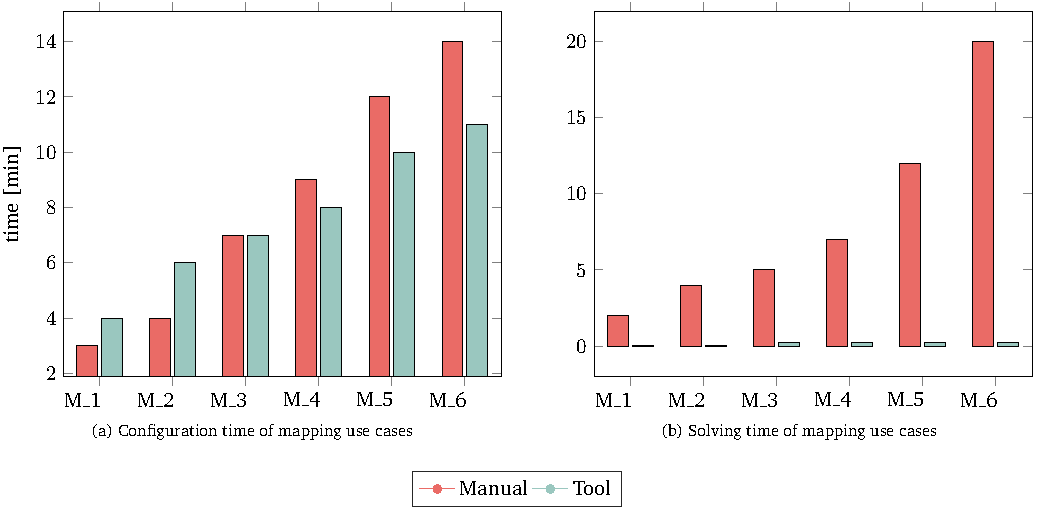
\includegraphics[width=1\textwidth]{figures/qual_mapping.pdf}}
	\caption{Results of the quantitative evaluation for the mapping case studies using a manual approach and the E/E Designer tool. (a) The required setup time for each use case. (b) The required solving time for each use case.}
	\label{mapping_use_cases_setup_time}
    \end{figure}
    
    %While, figure~\ref{fig:communication_topology}~(b) presents the solving for the mapping use cases using two approaches such as the manual and the tool. The solving time grows exponentially with increasing the number of components in the topologies when the case studies are manually solved by a person. Although, it is easy to intuitively find solutions for use cases with a few constraints, it becomes exponentially more difficult if the number of constraints increases.
    %Whereas, based on figure~\ref{mapping_use_cases_setup_time}~(b), the time for solving the same use cases using the tool remains extremely low and consistent compared to the manual approach. Even when scaling it to larger topologies, the required time for solving the constraint set of mapping does not increase relevantly. Moreover, adding further constraints does not show any significant impact on the solution time. This proves that how the proposed framework can facilitates the design process of vehicle E/E architectures.  
    In Figure~\ref{mapping_use_cases_setup_time}~(b), the mapping use cases are illustrated using two distinct approaches: manual and tool-assisted. It is noteworthy that the solving time exhibits exponential growth as the number of components in the topologies increases when these case studies are solved manually. While it may be relatively straightforward to intuitively derive solutions for use cases with a limited number of constraints, the complexity rises exponentially as the constraints multiply.
    In contrast, referring to Figure~\ref{mapping_use_cases_setup_time}~(b), the time required for solving these same use cases via the tool remains remarkably low and consistent in comparison to the manual method. This holds true even as the scale of topologies expands, with the time needed to solve the mapping constraint set remaining relatively unaffected. Furthermore, the addition of further constraints does not significantly impact the solution time. This serves as evidence of how the proposed framework adeptly streamlines the design process for vehicle E/E architectures.




    
    %Though, for the solution time, a significant and exponential speedup can be observed. For the manual solving, the required time increases exponentially for more ECUs and applications as the number of possible options increase significantly. While it is easy to intuitively find solutions for use cases with a few constraints, it becomes exponentially more difficult if the number of constraints increases.
    
    %Contrary, the solution time required by the framework stays very low and consistent, especially due to the single-step approach. Even when scaling it to larger use cases, the required time for constraint-restricted mapping does not increase relevantly. Moreover, adding further constraints does not show any significant impact on the solution time. 
    


    \subsubsection{Mapping \& Routing Case Studies}
    %In addition to the mapping use cases, also routing \& mapping use cases have been considered. These use cases aim to assess the overall functionality of the E/E Designer framework:
    In addition to the mapping use cases, routing and mapping use cases have also been taken into account. These specific use cases serve the purpose of comprehensively evaluating the overall functionality of the E/E Designer framework. The following case studies are considered and given to a group of students to perform the quantitative and qualitative analysis similar to the mapping case studies.
    \begin{itemize}
        \item M\&R\_1: 5 ECUs, 2 applications with up to one thread, 1 communication message
        \item M\&R\_2: 5 ECUs, 8 applications with up to two threads, 4 communication messages
        \item M\&R\_3: 5 ECUs, 12 applications with up to two threads, 6 communication messages
        \item M\&R\_4: 5 ECUs, 16 applications with up to two threads, 8 communication messages
        \item M\&R\_5: 5 ECUs, 20 applications with up to two threads, 10 communication messages
        \item M\&R\_6: 5 ECUs, 28 applications with up to two threads, 14 communication messages
        \item M\&R\_7: 5 ECUs, 74 applications with up to two threads, 37 communication messages
    \end{itemize}

    %For solving the routing\&mapping use cases, the subsequent constraints have been considered:
    To handle the routing and mapping use cases, the following constraints have been taken into account.
    \begin{itemize}
        \item Scheduling constraints for applications threads and communication tasks
        \item Message routing conditions to find a reliable path from a sender to a receiver
        \item Each ECU must execute at least one application
        \item Each LOR's link must be maximum three
    \end{itemize}
    Moreover, within the solving process, the optimization objectives of end-to-end latency and response time are duly taken into account.

    
    %The figure~\ref{qual_routing}~(a) expresses the configuration times for designing the above-discussed mapping \& routing case studies using manual and tool-assisted approaches. Similar to the mapping experiment, in small scale, the modeling by the framework takes more time than the manual approach; however, as soon as the size of model grows, using the tool makes the design process faster as can be observed in figure~\ref{qual_routing}~(a). The solving process of the mapping \& routing experiment takes much longer than the mapping experiment both using the manual solving, as can be perceived in  figure~\ref{qual_routing}~(b). The main reasons are the required optimization goals as well as the number of problems that needs to be solved. Moreover, there is a significant difference in solving time between using the manual and tool approaches. It should be added that in the manual solving time the optimality of the solutions as well as their visualizations were not considered. These comparisons clearly show that the E/E designer yields significant improvements for setting up but especially for solving use cases from quantitative point of view.
    
    Figure~\ref{qual_routing}~(a) expresses the configuration times associated with the design of the mapping and routing case studies illustrated above using both manual and tool-assisted approaches. In parallel to the mapping experiment, the framework's modeling process consumes more time at a smaller scale than the manual approach. However, as the model size increases, the utilization of the tool becomes advantageous, resulting in an expedited design process, as evident in Figure~\ref{qual_routing}~(a).
    
     \begin{figure}[t]
	\centering
	\makebox[\textwidth][c]{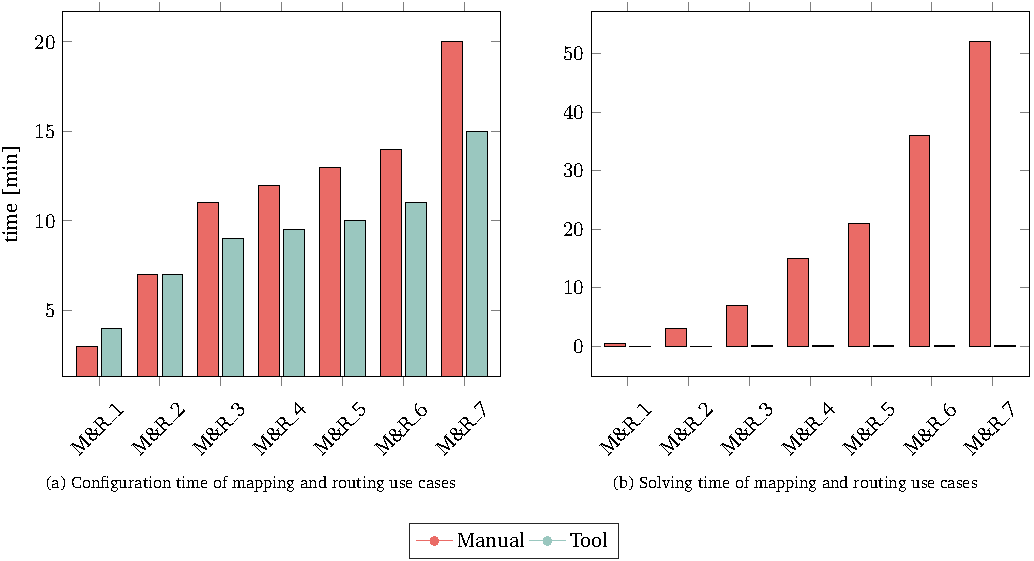
\includegraphics[width=1\textwidth]{figures/qual_mapp_route.pdf}}
	\caption{ 
    Results of the quantitative evaluation for the mapping and routing case studies using manual and tool-assisted approaches. (a) The required setup time for each use case. (b) The required solving time for each use case. The manual solving time does not include visualization and optimality of the solutions.}
	\label{qual_routing}
    \end{figure}
    
    The solving process of the mapping and routing experiment demonstrates significantly longer durations than the mapping experiment within the manual solving, as illustrated in Figure~\ref{qual_routing}~(b). The extended durations can be attributed to the complexity introduced by optimization goals and the number of problems necessitating resolution. 
    Moreover, as can be seen, there is a significant difference in solving time between using the manual and tool-based approaches.
    %Notably, a notable disparity in solving time exists between the manual and tool-based approaches.
    It should be added that the manual solving time does not account for solution optimality or visualization. The comparisons drawn here distinctly emphasize the pronounced enhancements offered by the proposed framework, not only in the setup but particularly in the resolution of use cases, from a quantitative standpoint. These insights underscore the tool's efficacy and efficiency in navigating intricate design scenarios.
  
    %The subsequent figures show the setup time as well as the solution time for the different mapping+routing use cases.
    

   

    
    %As it can be seen from the measured timing, the achieved speed-up for the mapping+routing use cases is very large. The main reason for the long manual solving times are the required optimization goals as well as the exponential growing number of possible solutions. 
    
    
   
    
    %These comparisons clearly show that the E/E designer yields significant improvements for setting up but especially for solving use cases from qualitative and quantitative point of view.

    \subsection{Qualitative Analysis}

    %Apart from the mentioned quantitative and measurable advantages, there are also qualitative differences between the manual results and the solutions of the E/E Designer.First of all, the manual solving has to be re-done completely as soon as one object property changes. While it also has to be solved again for the E/E Designer, it is obvious that trying out different properties can be done multiple times faster by using the framework. Additionally, the tool provides a fast overview whether the desired configuration is possible at all. For the manual approach, all possible combinations need to be checked in order to decide that. This could be sped up as soon as partial mappings are violating the constraints. Though, it requires a significant extra time to verify it.
    
    In addition to the quantifiable benefits, qualitative distinctions exist between the outcomes of manual approaches and the solutions offered by the introduced tool.
    \begin{itemize}
        \item The manual solving process necessitates a complete restart whenever a single object property changes. While the need to re-solve remains applicable to the introduced framework's approach, it is evident that the framework enables rapid exploration of various property permutations. This accelerated process is an important advantage.
        \item The tool swiftly offers an overview of the feasibility of a desired configuration. Conversely, the manual method mandates a comprehensive exploration of all feasible combinations, a time-consuming task. This process can potentially be expedited when partial mappings breach the constraints. Nevertheless, validating this condition requires substantial additional time.
        \item The visualization of results quickly becomes disorganized when manual mapping is carried out. In contrast, the E/E Designer automatically presents the outcomes in a visually coherent manner, adeptly avoiding the issue of overlapping visuals.
        \item  The E/E Designer offers a significant advantage. The tool ensures the finding of an optimal solution. In contrast, when attempting manual solutions, especially for more extensive use cases, it is possible to find solutions; however, discovering the optimized solution becomes exceedingly challenging or unattainable.
    \end{itemize}
     
    %\null
    %\addtocounter{page}{1}
    %\newpage
    %\thispagestyle{empty}
    
    %The visualization of the results becomes unstructured very fast when manual mapping is performed. Contrary, the E/E Designer automatically shows the result in visually comfortable way, i.e. by avoiding overlapping of visuals.



    
    %Additionally, there is an important advantage of the E/E Designer. The tool guarantees to find the optimal solution. For the manual solving, especially for the larger use cases, it was possible to find solutions but it is very difficult or not possible at all to find the optimal solution. 

    \begin{comment}
    
    \subsubsection{Expert Interviews}
    
    The expert interviews have been conducted with multiple E/E developers, architects, and managers from different automotive OEMs and suppliers.
    The experts provided feedback on the usability, the already integrated functionalities as well as the practicability of generated solutions.
    In addition, general research has been conducted to assess the different categories.

    \textbf{Usability}
    The conducted user studies have shown that the tool is very intuitive to use. The users are able to quickly grasp where information is located and how to add and adapt new objects. 
    Though, one drawback that has been observed multiple is the intuitivity of how to analyse the results. While the general solution can be understood easily, it was complicated for the users to figure out where and how they can analyze the scheduling. 
    Finally, solving the use cases is very comfortable apart from one drawback: If a use case is solvable, the experts need to see the specific reasons and maybe even possible solutions in order to adapt it.

    \textbf{Functionalities}
    As already stated in the beginning, the expert interviews have been very supportive to add and adapt constraints and optimization goals of the E/E Designer. This section focuses on the evaluation of the implemented constraints. Overall, the implemented functionalities have been evaluated very positively. However, there are many edge cases that are not yet considered for 


    \textbf{Practicability of solutions}
    The generated solutions look valid and reasonable to the experts. As it was also already identified during the requirements analysis, for practicability, it is necessary that there are multiple proposed solutions which also include key metrics like costs, and overall latency.
    It is mentioned very positively, that the framework allows easy adaptation of use cases and to continue working on the E/E architecture based on the outcome of the framework. 
    
        \end{comment}

    
    